%% main.tex — ISSRE 2026 camera-ready (RES track, 12 pages incl. references).
\documentclass[conference]{IEEEtran}

%% ----- Packages -----
\usepackage{amsmath,amssymb,amsthm}
\usepackage{mathtools}
\usepackage{enumerate}
\usepackage{graphicx}
\usepackage{booktabs}
\usepackage{array}
\usepackage{hyperref}
\usepackage[table]{xcolor}
\usepackage{microtype}
\usepackage{balance}
\usepackage{tikz}
\usepackage[misc]{ifsym}
\usetikzlibrary{arrows.meta, positioning, shapes.geometric, fit, backgrounds}
\usepackage[ruled,linesnumbered]{algorithm2e}
\newcommand{\AlgoCommentSty}[1]{\textcolor{blue!55!black}{\scriptsize\emph{#1}}}
\SetCommentSty{AlgoCommentSty}
\definecolor{TableHeader}{RGB}{232,238,247}
\definecolor{TableStripe}{RGB}{247,249,252}
\definecolor{TableHighlight}{RGB}{232,246,238}
\definecolor{TableRule}{RGB}{120,130,145}
\newcommand{\theadrow}{\rowcolor{TableHeader}}
\newcommand{\tstriped}{\rowcolor{TableStripe}}
\newcommand{\thighlight}{\rowcolor{TableHighlight}}

%% ----- Theorem environments -----
\newtheorem{theorem}{Theorem}
\newtheorem{proposition}[theorem]{Proposition}
\newtheorem{lemma}[theorem]{Lemma}
\newtheorem{corollary}[theorem]{Corollary}
\newtheorem{definition}{Definition}
\newtheorem{assumption}{Assumption}
\newtheorem{remark}[theorem]{Remark}

%% ----- Custom commands -----
\newcommand{\R}{\mathcal{R}}
\newcommand{\Rinf}{R_{\infty}}
\newcommand{\ST}{\mathcal{S}_T}
\newcommand{\Sset}{\mathcal{S}}
% \newcommand{\succ}{\oplus}
\newcommand{\fail}{\ominus}
\newcommand{\Nmat}{N}
\newcommand{\ones}{\mathbf{1}}
\newcommand{\Rsucc}{R_{\oplus}}
\newcommand{\Rfail}{R_{\ominus}}

\IEEEoverridecommandlockouts

\begin{document}

\title{\textsc{TraceToChain}: Auditing LLM-Agent Reliability with Absorbing Markov Chains}

\author{\IEEEauthorblockN{Phat T. Tran-Truong \href{https://orcid.org/0000-0003-3199-6333}{
\includegraphics[scale=0.004]{sugg.png}}, Xuan-Bach Le$^{\text{(\Letter)}}$ \href{https://orcid.org/0009-0003-6848-5403}{
\includegraphics[scale=0.004]{sugg.png}}}
\IEEEauthorblockA{\textit{Faculty of Computer Science and Engineering} \\
\textit{Ho Chi Minh City University of Technology (HCMUT), VNU-HCM}\\
Ho Chi Minh City, Vietnam \\
\{phatttt, lexuanbach\}@hcmut.edu.vn}
}


\maketitle
\bstctlcite{BSTcontrol}
\begingroup\renewcommand\thefootnote{}
\footnotetext{
$^{\text{(\Letter)}}$ Corresponding Author: Xuan-Bach Le (lexuanbach@hcmut.edu.vn)\\
Artifact: \url{https://github.com/lexuanbach/TraceToChain}
}
\endgroup

\begin{abstract}
Large language model (LLM) agents are sequential software systems, yet
their reliability is reported as scalar benchmark scores---pass$@k$,
pass$^k$, and the reliability decay curve (RDC)---that neither identify
the success-time distribution being estimated nor test whether traces support
it, leaving horizon, counterfactual, and metric-reconciliation
questions unanswerable. We present
\textsc{TraceToChain}, a reproducible pipeline that fits agent traces to
an absorbing discrete-time Markov chain by Laplace-smoothed maximum
likelihood, gates every result behind a composite Akaike
information criterion and Kolmogorov--Smirnov (KS) certificate, and
attaches Dirichlet-posterior and bootstrap intervals. We evaluate it under a strict 50/50 fit/test
protocol on seven controlled MAST-style corpora and on $2{,}459$ real
episodes: $479$ SWE-bench~Verified SWE-agent trajectories and $1{,}980$
$\tau$-bench episodes over two models and two domains. On
held-out controlled traces the fitted chain reproduces the RDC to a
maximum $L_\infty$ error of $0.053$ and passes the first-passage KS
test on $7/7$ frameworks (minimum $p=0.83$). On real
traces the certified asymptotic reliability recovers the held-out pass
rate to within $0.03$ on SWE-bench and to a mean absolute error of
$0.0075$ across four $\tau$-bench corpora, and one fitted chain yields
pass$@k$, pass$^k$, and closed-form perturbation answers
($\Delta R_\infty = +0.034$ for a fallback tool) with no benchmark
rerun. The certificate states exactly which outputs the
evidence supports, and its verdict is invariant across $18$ clustering
configurations of the real corpus. LLM-agent reliability engineering
can thus move from scalar scores to an audited model that identifies
its own trustworthy outputs.
\end{abstract}

\begin{IEEEkeywords}
software reliability, large language models, agent systems,
absorbing Markov chains, goodness-of-fit, model auditing, first-passage time,
pass@k, reliability decay curve
\end{IEEEkeywords}

%% ================================================================

\section{Introduction}
\label{sec:intro}

%% --- 1. Context -------------------------------------------------
Large language model (LLM) agents now run as sequential software
systems in production: a deployed agent plans, calls tools, observes
results, retries, and terminates in success or failure, as in
ReAct-style and tool-using
designs~\cite{yao2023react,schick2023toolformer,wang2024agentsurvey}.
Once such an agent sits on a critical path---resolving a support
ticket, patching a repository, issuing a refund---the operator inherits
the ordinary obligations of dependability and site reliability
engineering (SRE)~\cite{avizienis2004dependability,beyer2016sre}:
state a reliability target, quantify the uncertainty around it, and say
under what conditions it holds.

%% --- 2. Narrow to the specific problem --------------------------
Agent evaluation, however, reports reliability as a scalar. Benchmarks
supply rich execution traces---ToolBench~\cite{qin2023toolllm},
$\tau$-bench~\cite{taub2024}, SWE-bench~\cite{swebench2024},
WebArena~\cite{zhou2023webarena}, and
AgentBench~\cite{agentbench2024}---but summarize them as
pass$@k$~\cite{chen2021codex}, pass$^k$, or the reliability decay curve
(RDC)~\cite{rdc2025}. Each score is a different summary of when a run
succeeds, computed with a different denominator and reported without a
fit check. Classical software reliability already has the machinery for
this setting, from Markov program models~\cite{cheung1980} and
absorbing chains~\cite{kemenysnell} to reliability-growth
models~\cite{goelokt,musa1987}, and trace-driven frameworks such as
TriCEGAR~\cite{tricegar2026} and ProbGuard~\cite{pro2guard2025} learn
Markov abstractions from execution data.

%% --- 3. The gap -------------------------------------------------
Despite this, no current LLM-agent reliability report names the
success-time distribution it estimates, tests whether the traces
support that distribution, or attaches finite-trace uncertainty to it.
The practical cost is concrete. A team that ships a refund agent at
$\mathrm{pass}@1 = 0.72$ cannot say what reliability a larger step
budget buys, what an added fallback tool changes end-to-end, or how an
internal $\mathrm{pass}^5$ dashboard relates to an SRE
mean-time-between-failures target---without rerunning the benchmark
once per question, and still without an interval or a validity check.

%% --- 4. Contribution --------------------------------------------
In this paper we propose \textsc{TraceToChain}, a pipeline that turns an
agent trace corpus into an \emph{audited} reliability model. Each
execution becomes a trajectory in an absorbing discrete-time Markov
chain (DTMC) $\hat M=(\ST,\hat Q,\hat R_\oplus,\hat R_\ominus,s_0)$
(Definition~\ref{def:amc}), with transient states $\ST$ for
intermediate behavior and absorbing states for terminal success and
failure. What distinguishes \textsc{TraceToChain}
from prior trace-to-DTMC abstraction is that the fit is not trusted by
default: a composite Akaike information criterion (AIC) and
Kolmogorov--Smirnov (KS) certificate gates every reported quantity, and
Dirichlet-posterior and bootstrap intervals accompany the ones that
pass. Horizon reliability, local perturbation, and metric
reconciliation then become first-passage queries on one model
(Props.~\ref{thm:closed} and~\ref{thm:perturb}, Thm.~\ref{thm:unify}),
so pass$@k$, pass$^k$, and the RDC stop competing and become
projections of a single success-time distribution.

%% --- 5. Approach and key results in brief -----------------------
Figure~\ref{fig:design} shows the pipeline and the study design that
evaluates it: a strict 50/50 fit/test protocol on seven controlled
MAST-style corpora, then end-to-end fits on $2{,}459$ real agent
episodes from two independent benchmarks. In both settings the
certified outputs track their held-out targets closely, and the
certificate marks precisely which further outputs its evidence
supports---the behavior a reliability audit is supposed to have.

%% --- 6. Explicit contributions ----------------------------------
Our contributions are:
\begin{enumerate}[(1)]
  \item \emph{An audited trace-to-chain pipeline.}
  \textsc{TraceToChain} (\S\ref{sec:state_construction},
  Algorithms~\ref{alg:trace}--\ref{alg:gof}) maps traces to a fitted
  absorbing DTMC behind a composite AIC$\,\wedge\,$KS goodness-of-fit
  certificate, with Dirichlet-posterior and trace-level bootstrap
  intervals on the chain and every derived quantity (\S\ref{sec:uq}).
  \item \emph{Metric unification.}
  pass$@k$, pass$^k$, and the RDC are derived as projections of one
  success first-passage distribution (Thm.~\ref{thm:unify}), making
  their denominators explicit and their disagreement resolvable.
  \item \emph{Held-out validation.}
  On seven controlled MAST-style frameworks (SS9, \S\ref{sec:ss9}) the
  pipeline attains maximum RDC error
  $L_\infty^{\mathrm{RDC}}=0.053$ (median $0.048$) and held-out KS
  $p>0.05$ on $7/7$ frameworks (min $p=0.83$).
  \item \emph{Real-trace validation on two benchmarks.}
  Fitting end-to-end to $479$ SWE-bench~Verified SWE-agent trajectories
  (SS10--SS14, \S\ref{sec:ss10}) and $1{,}980$ $\tau$-bench episodes
  (SS15, \S\ref{sec:ss15}) recovers the held-out pass rate to within
  $0.03$ and to a mean of $0.0075$ respectively, delivering
  metric-reconciliation and closed-form perturbation answers on real
  agents while the audit scopes the remaining outputs.
  \item \emph{Sensitivity analysis.}
  Clustering, censoring, and bootstrap-path studies
  (SS11--SS13, \S\ref{sec:robustness}) show the verdict is invariant
  across $18$ clustering configurations, and that $\hat R_\infty$ stays
  within $4\%$ of a synthetic ground truth up to $50\%$ censoring.
\end{enumerate}

%% --- 7. Roadmap -------------------------------------------------
The rest of this paper is organized as follows.
\S\ref{sec:related} positions the work; \S\ref{sec:formal} and
\S\ref{sec:state_construction} define and fit the absorbing-chain
model; \S\ref{sec:core} and \S\ref{sec:ext} derive the reliability
results; \S\ref{sec:sim}--\S\ref{sec:robustness} report the controlled,
real-trace, and sensitivity studies; and
\S\ref{sec:threats}--\S\ref{sec:conc} discuss limits and implications.

\begin{figure}[!t]
\centering
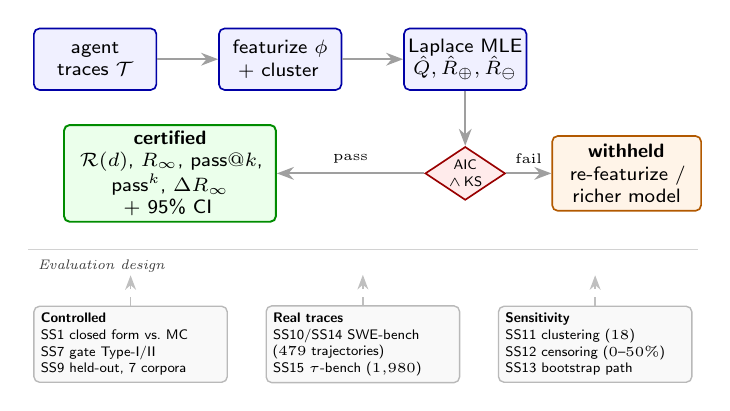
\begin{tikzpicture}[
  >=Stealth, font=\scriptsize\sffamily,
  st/.style={rectangle, rounded corners=2pt, draw=blue!65!black, fill=blue!6,
             line width=0.6pt, align=center, text width=1.45cm,
             minimum height=0.78cm, inner sep=1.5pt},
  gate/.style={diamond, aspect=1.5, draw=red!60!black, fill=red!8,
               line width=0.6pt, align=center, inner sep=0.5pt, font=\tiny\sffamily},
  good/.style={rectangle, rounded corners=2pt, draw=green!55!black, fill=green!8,
               line width=0.7pt, align=center, text width=2.55cm,
               minimum height=0.95cm, inner sep=2pt},
  bad/.style={rectangle, rounded corners=2pt, draw=orange!70!black, fill=orange!9,
              line width=0.6pt, align=center, text width=1.75cm,
              minimum height=0.95cm, inner sep=2pt},
  ev/.style={rectangle, rounded corners=2pt, draw=gray!55, fill=gray!5,
             line width=0.5pt, align=left, text width=2.28cm, inner sep=2.5pt,
             font=\tiny\sffamily},
  ar/.style={->, draw=gray!75, line width=0.7pt},
  dar/.style={->, draw=gray!50, line width=0.5pt, dashed, shorten >=1pt}]
  \node[st] (tr)  at (0.80, 0)     {agent\\traces $\mathcal T$};
  \node[st] (fe)  at (3.15, 0)     {featurize $\phi$\\+ cluster};
  \node[st] (mle) at (5.50, 0)     {Laplace MLE\\$\hat Q,\hat R_\oplus,\hat R_\ominus$};
  \node[gate] (g) at (5.50, -1.45) {AIC\\$\wedge$\,KS};
  \node[good] (ok) at (1.75, -1.45)
      {\textbf{certified}\\$\mathcal R(d)$, $R_\infty$, pass$@k$,\\pass$^k$, $\Delta R_\infty$ $+$ 95\% CI};
  \node[bad] (no) at (7.55, -1.45) {\textbf{withheld}\\re-featurize /\\richer model};
  \draw[ar] (tr) -- (fe);
  \draw[ar] (fe) -- (mle);
  \draw[ar] (mle) -- (g);
  \draw[ar] (g) -- node[above, font=\tiny] {pass} (ok);
  \draw[ar] (g) -- node[above, font=\tiny] {fail} (no);
  \draw[gray!35, line width=0.4pt] (-0.05,-2.42) -- (8.45,-2.42);
  \node[anchor=west, font=\tiny\itshape, text=gray!45!black]
       at (-0.05,-2.63) {Evaluation design};
  \node[ev] (e1) at (1.25, -3.62)
      {\textbf{Controlled}\\SS1 closed form vs.\ MC\\SS7 gate Type-I/II\\SS9 held-out, 7 corpora};
  \node[ev] (e2) at (4.20, -3.62)
      {\textbf{Real traces}\\SS10/SS14 SWE-bench\\($479$ trajectories)\\SS15 $\tau$-bench ($1{,}980$)};
  \node[ev] (e3) at (7.15, -3.62)
      {\textbf{Sensitivity}\\SS11 clustering ($18$)\\SS12 censoring ($0$--$50\%$)\\SS13 bootstrap path};
  \draw[dar] (e1.north) -- ++(0,0.42);
  \draw[dar] (e2.north) -- ++(0,0.42);
  \draw[dar] (e3.north) -- ++(0,0.42);
\end{tikzpicture}
\caption{\textsc{TraceToChain} pipeline and evaluation design.}
\label{fig:design}
\end{figure}

%% [REDUCTION] The three-column motivating figure is suppressed for the
%% 12-page body; the paragraph above states Q1--Q3 and points at the
%% results that answer them. Retained in source for the artifact.
\iffalse
\begin{figure}[!t]
\centering
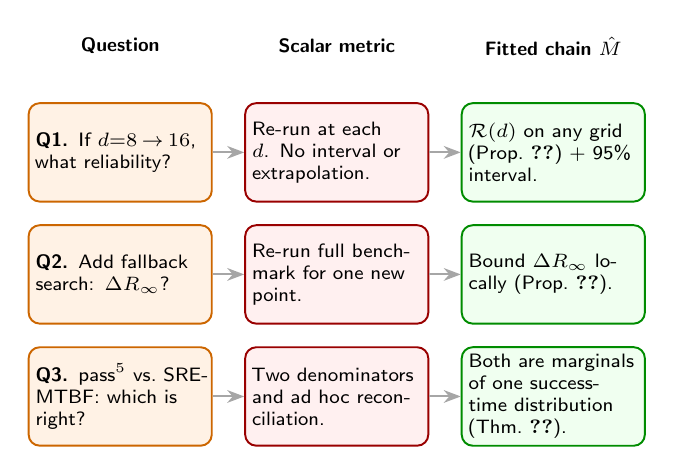
\begin{tikzpicture}[
    >=Stealth,
    font=\scriptsize\sffamily,
    hdr/.style={font=\bfseries\sffamily\scriptsize, align=center},
    q/.style={rectangle, rounded corners, draw=orange!80!black,
              fill=orange!10, line width=0.7pt, align=left,
              text width=2.15cm, inner sep=2.5pt, minimum height=1.25cm},
    s/.style={rectangle, rounded corners, draw=red!60!black,
              fill=red!6, line width=0.7pt, align=left,
              text width=2.15cm, inner sep=2.5pt, minimum height=1.25cm},
    a/.style={rectangle, rounded corners, draw=green!55!black,
              fill=green!6, line width=0.7pt, align=left,
              text width=2.15cm, inner sep=2.5pt, minimum height=1.25cm},
    lbl/.style={font=\scriptsize\itshape, text=gray!50!black},
    arr/.style={->, draw=gray!70, line width=0.7pt},
    xscale=1.0, yscale=1.0,
]
    % column centers
    \def\colQ{0}
    \def\colS{2.75}
    \def\colA{5.5}
    % row y-coordinates
    \def\rowH{0.85}
    \def\rowA{-0.5}
    \def\rowB{-2.05}
    \def\rowC{-3.6}

    % Headers
    \node[hdr] at (\colQ, \rowH)
        {Question};
    \node[hdr] at (\colS, \rowH)
        {Scalar metric};
    \node[hdr] at (\colA, \rowH)
        {Fitted chain $\hat M$};

    % Row 1: budget
    \node[q] (q1) at (\colQ, \rowA)
        {\textbf{Q1.} If $d{=}8\!\to\!16$, what reliability?};
    \node[s] (s1) at (\colS, \rowA)
        {Re-run at each $d$. No interval or extrapolation.};
    \node[a] (a1) at (\colA, \rowA)
        {$\mathcal R(d)$ on any grid
         (Prop.~\ref{thm:closed}) + 95\% interval.};

    % Row 2: fallback tool
    \node[q] (q2) at (\colQ, \rowB)
        {\textbf{Q2.} Add fallback search: $\Delta R_\infty$?};
    \node[s] (s2) at (\colS, \rowB)
        {Re-run full benchmark for one new point.};
    \node[a] (a2) at (\colA, \rowB)
        {Bound $\Delta R_\infty$
         locally (Prop.~\ref{thm:perturb}).};

    % Row 3: metric zoo
    \node[q] (q3) at (\colQ, \rowC)
        {\textbf{Q3.} pass$^5$ vs.\ SRE-MTBF: which is right?};
    \node[s] (s3) at (\colS, \rowC)
        {Two denominators and ad hoc reconciliation.};
    \node[a] (a3) at (\colA, \rowC)
        {Both are marginals of one success-time distribution
         (Thm.~\ref{thm:unify}).};

    \draw[arr] (q1) -- (s1);
    \draw[arr] (s1) -- (a1);
    \draw[arr] (q2) -- (s2);
    \draw[arr] (s2) -- (a2);
    \draw[arr] (q3) -- (s3);
    \draw[arr] (s3) -- (a3);
\end{tikzpicture}
\caption{Motivating example: a fitted absorbing chain turns one trace
         corpus into horizon, perturbation, and metric-reconciliation
         queries.}
\label{fig:motivating}
\end{figure}
\fi


%% ----------------------------------------------------------------
%% [REDUCTION 2026-04-24] Expanded contributions block retained
%% for the artifact but replaced above with a prose paragraph
%% to save ~30 lines in the 12-page body.
%% ----------------------------------------------------------------
\iffalse
\begin{enumerate}[(C1)]
  \item \emph{\textsc{TraceToChain} pipeline and goodness-of-fit
        certificate} (\S\ref{sec:state_construction},
        Algorithms~\ref{alg:trace}--\ref{alg:gof}): agglomerative
        Ward clustering with silhouette-chosen $m$, Laplace-smoothed
        MLE with explicit time-homogeneity, variable-horizon, and
        right-censoring semantics, plus a composite AIC$\,\wedge\,$KS
        test that certifies whether an agent trace corpus is
        adequately modeled by a first-order absorbing DTMC.
  \item \emph{Uncertainty quantification}
        (\S\ref{sec:uq}, \texttt{mcr.uncertainty}): closed-form
        Dirichlet posterior credible intervals on every entry of
        $\hat Q, \hat R_\oplus, \hat R_\ominus$ (Beta-marginal
        Dirichlet-Multinomial conjugacy) plus a trace-level
        non-parametric bootstrap. Every downstream reliability
        quantity inherits a calibrated CI.
  \item \emph{Held-out empirical validation}
        (\S\ref{sec:ss7}, \S\ref{sec:mast}): we fit on a
        randomly-sampled half of each framework's MAST-derived
        corpus and report, on the truly held-out half, (i)~the
        empirical RDC overlaid on the analytic $\mathcal R(d)$,
        (ii)~the Kolmogorov--Smirnov distance $D_{\mathrm{KS}}$ and
        $p$-value, and (iii)~the $L_\infty$ RDC error.
        SS7 additionally validates the Type-I/Type-II error of the
        composite test on synthetic chains with known ground truth.
  \item \emph{Metric unification} (Theorem~\ref{thm:unify},
        Corollary~\ref{cor:diag}): pass$@k$, pass$^k$, and the RDC
        are all restrictions of the same first-passage distribution.
        A correlated-trial correction gives a Jensen-gap diagnostic
        that flags when independent-trial assumptions fail.
  \item \emph{Classical analytic tools, application-layer}
        (Propositions~\ref{thm:closed}--\ref{thm:mixing}):
        closed-form $\mathcal R(d)$, $R_\infty$, and $\mathrm{MTTA}$;
        a condition-number sensitivity bound; RDC-shape sufficient
        conditions; the Goel--Okumoto NHPP limit; and a spectral
        horizon bound. Each is attributed and framed as an
        application of an established result.
  \item \emph{Reproducibility artifact}: the entire pipeline (six
        simulation studies, the MAST corpus, and all tables /
        figures in this paper) runs on a laptop in under
        $15$ minutes with a single command.
\end{enumerate}
\fi
%% ----------------------------------------------------------------


%% ================================================================
%% ----------------------------------------------------------------
%% [REDUCTION 2026-04-24] The standalone "Motivating Example"
%% section is commented out because \S I already contains a compact
%% motivating vignette and the 3-column figure (fig:motivating).
%% The prose below is retained for artifact completeness but not
%% compiled into the 12-page body.
%% ----------------------------------------------------------------
\iffalse
\section{Motivating Example: The On-Call Engineer}
\label{sec:motivating}

Consider a fintech that deploys a customer-refund agent built on a ReAct-style loop (plan $\to$ tool\_call $\to$ observe $\to$ reflect $\to$ answer). Before launch, the team reports a single headline number from the $\tau$-bench suite: $\mathrm{pass}@1 = 0.72$. Two weeks into production, an on-call engineer faces three routine questions:

\begin{enumerate}
    \item \emph{``If we raise the per-session step budget from 8 to 16, what reliability should we expect?''} The published $\mathrm{pass}@1$ is a single scalar; it says nothing about $\Pr[\tau_\oplus \leq d]$ for varying $d$. The team re-runs $\tau$-bench at $d{=}16$ on a laptop overnight and gets $0.77$, but cannot put a confidence interval on that number or extrapolate to $d{=}24$.

    \item \emph{``We added a fallback search tool; by how much does this change end-to-end reliability?''} Under the status quo this requires re-running the full benchmark. There is no perturbation estimator that translates a local change in one row of the transition matrix into an $R_\infty$ delta, because there is no transition matrix --- only an aggregate pass rate.

    \item \emph{``Our internal evaluation reports $\mathrm{pass}^k = 0.51$ at $k{=}5$, but the SRE dashboard expects an MTBF-style metric. Which is right?''} The engineer has two metrics computed by two teams with different denominators and cannot reconcile them without introducing yet a third.
\end{enumerate}

What unifies all three failures is that the community currently reports \emph{summary statistics of a first-passage distribution it never writes down.} $\mathrm{pass}@k$, $\mathrm{pass}^k$, and the RDC are three restrictions of one object --- $F_{\tau_\oplus}$ under the absorbing chain $\hat M = (\hat Q, \hat R_\oplus, \hat R_\ominus)$ --- but each benchmark reports only one restriction and each does so without an uncertainty interval, without a goodness-of-fit diagnostic, and without any lever the engineer can pull to ask ``what if.''

Our framework eliminates all three pain points by making $\hat M$ an \emph{explicit, audited artifact}:

\begin{itemize}
    \item \textbf{Unified first-passage view} (Theorem~\ref{thm:unify}). $\mathrm{pass}@k$, $\mathrm{pass}^k$, and $\mathcal{R}(d)$ are all read off from $F_{\tau_\oplus}$. The ``is $\mathrm{pass}@1$ or $\mathrm{pass}^k$ right?'' question becomes vacuous --- they answer different marginals of the same distribution.
    \item \textbf{Perturbation bound} (Proposition~\ref{thm:perturb}). A row-rank change $\Delta Q$ propagates to $\Delta R_\infty$ in closed form via $N = (I - \hat Q)^{-1}$; the fallback-tool question is answered in milliseconds without rerunning the benchmark.
    \item \textbf{Uncertainty quantification} (\S\ref{sec:uq}). Every entry of $\hat M$ carries a 95\% Dirichlet-posterior interval, which propagates to every downstream quantity, so the laptop-overnight $0.77$ comes with a calibrated CI.
    \item \textbf{Held-out goodness-of-fit} (SS9). If the agent's traces \emph{are not} adequately Markov on this corpus, the composite AIC $\wedge$ KS certificate rejects $\hat M$ --- and the engineer is told, with a quantitative $L_\infty^{\mathrm{RDC}}$ error and a held-out $p$-value, exactly how much to trust the answers above.
\end{itemize}

In short: the engineer does not currently have a vocabulary in which these three questions are answerable; after fitting one chain, they do. Figure~\ref{fig:motivating_example} illustrates this dilemma.

\begin{figure}[!t]
  \centering
  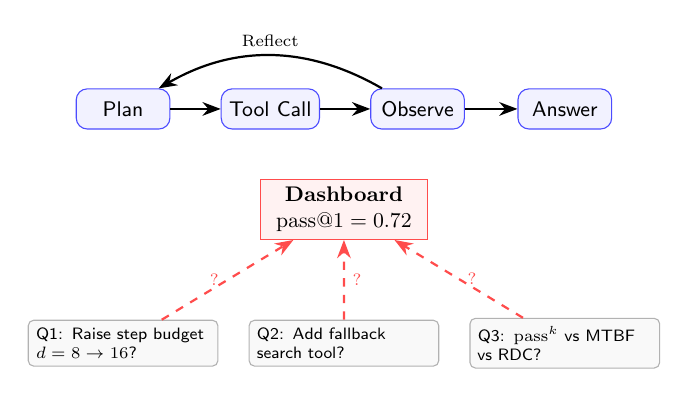
\begin{tikzpicture}[
      >=Stealth,
      scale=0.85, every node/.style={transform shape},
      box/.style={rectangle, draw=blue!70, fill=blue!5, rounded corners, align=center, font=\small\sffamily, minimum width=1.4cm, minimum height=0.6cm},
      metric/.style={rectangle, draw=red!70, fill=red!5, align=center, font=\bfseries\small, minimum width=2.5cm, minimum height=0.8cm},
      question/.style={rectangle, draw=gray!60, fill=gray!5, align=left, font=\scriptsize\sffamily, text width=2.6cm, rounded corners=2pt}
  ]
      % ReAct Loop
      \node[box] (plan) at (0, 0) {Plan};
      \node[box] (tool) at (2.2, 0) {Tool Call};
      \node[box] (obs)  at (4.4, 0) {Observe};
      \node[box] (ans)  at (6.6, 0) {Answer};
      
      \draw[->, thick] (plan) -- (tool);
      \draw[->, thick] (tool) -- (obs);
      \draw[->, thick] (obs) to[bend right=30] node[above, font=\scriptsize] {Reflect} (plan);
      \draw[->, thick] (obs) -- (ans);
      
      % Metric Dashboard
      \node[metric] (pass) at (3.3, -1.5) {Dashboard\\ $\mathrm{pass}@1 = 0.72$};
      
      % Questions
      \node[question] (q1) at (0, -3.5) {Q1: Raise step budget $d=8 \to 16$?};
      \node[question] (q2) at (3.3, -3.5) {Q2: Add fallback search tool?};
      \node[question] (q3) at (6.6, -3.5) {Q3: $\mathrm{pass}^k$ vs MTBF vs RDC?};
      
      \draw[->, dashed, color=red!70, thick] (q1) -- (pass) node[midway, left, font=\scriptsize, color=red!70] {?};
      \draw[->, dashed, color=red!70, thick] (q2) -- (pass) node[midway, right, font=\scriptsize, color=red!70] {?};
      \draw[->, dashed, color=red!70, thick] (q3) -- (pass) node[midway, right, font=\scriptsize, color=red!70] {?};

  \end{tikzpicture}
  \caption{Motivating example: an on-call engineer observes a single aggregate scalar metric ($\mathrm{pass}@1 = 0.72$), which cannot answer counterfactual questions about step budgets, tool perturbations, or metric reconciliation.}
  \label{fig:motivating_example}
\end{figure}
\fi
%% ----------------------------------------------------------------
%% [END REDUCTION 2026-04-24 — standalone motivating example]
%% ----------------------------------------------------------------

%% ================================================================
\section{Related Work}
\label{sec:related}

Prior work provides the ingredients for deployment reliability
decisions but not their combination: reliability engineering
contributes the vocabulary, agent benchmarks the trace setting, and
probabilistic verification the model-based reasoning. The missing piece
is an audited fit from LLM-agent traces---a model with uncertainty,
diagnostics, and shared semantics for common metrics.

%% [REDUCTION] The full-width method-comparison table is suppressed for the
%% 12-page body; the three paragraphs below plus the positioning summary
%% state the same taxonomy. Retained in source for the artifact.
\iffalse
\begin{table*}[!t]
\centering
\caption{Comparison of \textsc{TraceToChain} with related evaluation
and verification frameworks.}
\label{tab:method-comparison}
\scriptsize
\setlength{\tabcolsep}{3pt}
\renewcommand{\arraystretch}{1.12}
\begin{tabular}{@{}>{\raggedright\arraybackslash}p{0.22\textwidth}
                >{\raggedright\arraybackslash}p{0.15\textwidth}
                >{\raggedright\arraybackslash}p{0.2\textwidth}
                >{\raggedright\arraybackslash}p{0.22\textwidth}
                >{\raggedright\arraybackslash}p{0.1\textwidth}@{}}
\toprule
\textbf{Approach} & \textbf{Input} & \textbf{Reliability semantics} &
\textbf{Diagnostics / uncertainty} & \textbf{LLM-agent fit} \\
\midrule
\mbox{Classical SRE / NHPP~\cite{cheung1980,goelokt}} &
Aggregate failures &
Growth / failure intensity &
Aggregate intervals, no trace states &
Indirect \\
\tstriped
\mbox{Agent benchmark metrics~\cite{chen2021codex,rdc2025}} &
Outcomes / traces &
Success, pass$@k$, pass$^k$, RDC &
Metric-specific, limited fit checks &
Direct / split \\
\mbox{PRISM / Storm~\cite{prism2011,storm2017}} &
User model &
PCTL queries &
Verification, no trace fitting &
Indirect \\
\tstriped
\mbox{TriCEGAR / ProbGuard~\cite{tricegar2026,pro2guard2025}} &
Empirical traces &
Learned Markov abstraction &
Refinement diagnostics &
Related \\
\thighlight
\mbox{\textbf{\textsc{TraceToChain} (this work)}} &
\textbf{LLM-agent traces} &
\textbf{First-passage DTMC reliability} &
\textbf{AIC/KS diagnostics, posterior/bootstrap intervals} &
\textbf{Direct} \\
\bottomrule
\end{tabular}
\end{table*}
\fi


\paragraph{Classical SRE.}
Classical software reliability gives this paper its vocabulary and
analytic tools. The dependability taxonomy of Avi{\v z}ienis et al.\
separates reliability, availability, safety, and failure
semantics~\cite{avizienis2004dependability}, while SRE
practice~\cite{beyer2016sre} turns such concepts into measurable
service objectives. State-based modeling is equally central:
Cheung~\cite{cheung1980} used Markov chains for program-level software
reliability, Trivedi and Bobbio~\cite{trivedi2017reliability} give a
broader engineering treatment, and Kemeny and Snell~\cite{kemenysnell}
developed the absorbing-chain framework and fundamental matrix
$N=(I-Q)^{-1}$ used by our closed forms. Reliability-growth models add
a complementary aggregate view~\cite{goelokt,musa1987}. None of these
is by itself a trace-level evaluation method for LLM agents;
Proposition~\ref{thm:nhpp} connects them by recovering the NHPP form as
a rare-failure scaling limit of the fitted agent chain.

\paragraph{Agent benchmarks.}
Agent benchmarks show why trace-level reliability semantics are
needed. ReAct~\cite{yao2023react}, Toolformer~\cite{schick2023toolformer},
and Reflexion~\cite{shinn2023reflexion} established agent
trajectories that interleave reasoning, tool use, and revision steps;
ToolBench~\cite{qin2023toolllm} and $\tau$-bench~\cite{taub2024} make
API choice, tool errors, and tool-agent-user interaction part of the
evaluation surface. SWE-bench~\cite{swebench2024},
WebArena~\cite{zhou2023webarena}, ALFWorld~\cite{shridhar2021alfworld},
and Voyager~\cite{wang2023voyager} move evaluation further toward
software, web, embodied, and open-ended environments where success is
long-horizon and context-dependent. MAST~\cite{mast2025} diagnoses
multi-agent failure modes, and AgentBench~\cite{agentbench2024}
broadens the interactive evaluation space beyond one task family.
Together, these benchmarks expose the trace setting; they do not by
themselves unify the reported metrics. pass$@k$~\cite{chen2021codex}
originated as a repeated-sampling success metric for code generation,
and agent evaluation later adapted it alongside the reliability decay
curve (RDC)~\cite{rdc2025}, which tracks how repeated-trial reliability
\emph{degrades as task duration grows}. Our $d$-step reliability $R(d)$
(Definition~\ref{def:reliab}) is the complementary step-budget view: a
non-decreasing cumulative success probability indexed by the step
budget rather than a duration-indexed decay. We retain the RDC name for
continuity and state the modelled quantity explicitly in
\S\ref{sec:unify}.

\paragraph{Formal methods for agents.}
Formal methods supply the model-based reasoning layer. Probabilistic
computation tree logic (PCTL)~\cite{hansson1994pctl} supports
reasoning about probabilistic time and reliability properties, and
model-checking texts~\cite{baier2008principles} place such logics in a
broader verification framework. Given a probabilistic model,
PRISM~\cite{prism2011} and Storm~\cite{storm2017} can verify PCTL
properties. More recent trace-driven frameworks, including
TriCEGAR~\cite{tricegar2026} and ProbGuard~\cite{pro2guard2025}, learn
DTMC or Markov decision process (MDP) abstractions from empirical
traces. We therefore do not claim trace-to-DTMC abstraction as the
main theoretical novelty. Our focus is its reliability-engineering use
for LLM agents: \textsc{TraceToChain} fits an absorbing DTMC with a
composite AIC$\,\wedge\,$KS goodness-of-fit certificate and uncertainty
quantification, and SS9 (\S\ref{sec:ss9}) evaluates held-out recovery on
controlled MAST-style corpora using KS distance and
$L_\infty^{\mathrm{RDC}}$ error. The first-passage view explains why
pass$@k$, pass$^k$, and the RDC are restrictions of a single
distribution (Theorem~\ref{thm:unify}), while the Goel--Okumoto
NHPP appears as a rare-failure scaling limit of the fitted chain
(Proposition~\ref{thm:nhpp}).

\noindent\textbf{Positioning summary.}
These traditions are complementary rather than competing: classical
reliability models provide semantics, agent benchmarks provide traces,
and probabilistic-verification tools provide model-based queries, but
none of them fits and audits a reliability model from LLM-agent traces.
\textsc{TraceToChain}'s distinction is the
audited combination---traces define the estimate, diagnostics test the
abstraction, uncertainty bounds the reported quantities, and
first-passage semantics connect horizon reliability, perturbations, and
common LLM-agent metrics---which yields a reliability argument from
trace data rather than another scalar score.

%% ================================================================

\section{Formalism}
\label{sec:formal}

Deployment questions require probabilities that can be interpreted from
traces. The operational question is simple: after an agent has spent
several steps reasoning, calling tools, and observing outputs, what is
the probability that it reaches success before failure? We represent
that ``think-act-observe'' loop with a fitted absorbing discrete-time
Markov chain (DTMC), following classical absorbing-chain and
software-reliability models~\cite{kemenysnell,cheung1980}: intermediate
behavior becomes transient execution states, the two terminal outcomes
are task success~$\oplus$ and fatal failure~$\ominus$, and reliability
becomes a first-passage question---how soon a run reaches the success
absorber, and whether failure arrives first. This view also
gives benchmark metrics a common semantics, since
pass$@k$~\cite{chen2021codex}, pass$^k$~\cite{taub2024}, and the
step-budget reliability decay curve (RDC) in the sense of
\S\ref{sec:unify}~\cite{rdc2025} are all restrictions of one success
first-passage distribution. We write $\ST$ for the transient state set: the discrete
labels used for intermediate reasoning, tool-use, and observation
behavior before a run absorbs into $\oplus$ or $\ominus$.

%% [REDUCTION] fig:concept_translation is suppressed for the 12-page body:
%% Definition~\ref{def:amc} and Fig.~\ref{fig:pipeline} carry the model.
%% Retained in source for the artifact.
\iffalse
\begin{figure}[!t]
  \centering
  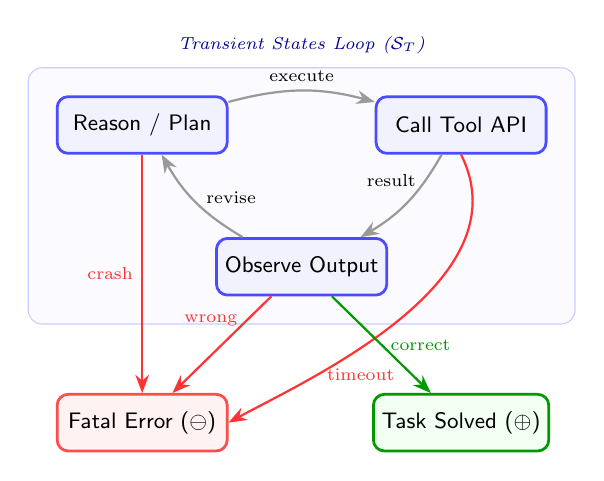
\begin{tikzpicture}[
      >=Stealth,
      scale=0.9, every node/.style={transform shape},
      concept/.style={rectangle, rounded corners, draw=blue!70, fill=blue!5, line width=1pt, align=center, font=\small\sffamily, minimum width=2.4cm, minimum height=0.8cm},
      success/.style={rectangle, rounded corners, draw=green!60!black, fill=green!5, line width=1pt, align=center, font=\small\sffamily, minimum width=2.4cm, minimum height=0.8cm},
      fail/.style={rectangle, rounded corners, draw=red!70, fill=red!5, line width=1pt, align=center, font=\small\sffamily, minimum width=2.4cm, minimum height=0.8cm},
      trans/.style={->, draw=gray!80, line width=0.8pt, font=\scriptsize}
  ]
      % Transient nodes
      \node[concept] (plan) at (0, 0) {Reason / Plan};
      \node[concept] (tool) at (4.5, 0) {Call Tool API};
      \node[concept] (obs) at (2.25, -2) {Observe Output};
      
      % Absorbing nodes
      \node[fail] (fail1) at (0, -4.2) {Fatal Error ($\ominus$)};
      \node[success] (succ) at (4.5, -4.2) {Task Solved ($\oplus$)};
      
      % Transient edges
      \draw[trans] (plan) to[bend left=15] node[above] {execute} (tool);
      \draw[trans] (tool) to[bend left=15] node[left, near start] {result} (obs);
      \draw[trans] (obs) to[bend left=15] node[right, pos=0.55, xshift=2pt] {revise} (plan);
      
      % Absorbing edges
      \draw[trans, color=red!80] (plan) -- node[left] {crash} (fail1);
      \draw[trans, color=red!80] (tool.south) .. controls +(0.9,-1.8) and +(1.1,0.6) .. node[right, pos=0.72] {timeout} (fail1.east);
      \draw[trans, color=red!80] (obs) -- node[left, near start] {wrong} (fail1);
      \draw[trans, color=green!60!black] (obs) -- node[right] {correct} (succ);
      
      % Background box
      \begin{scope}[on background layer]
          \node[draw=blue!20, fill=blue!2, rounded corners=5pt, fit=(plan)(tool)(obs), inner sep=10pt] (tbox) {};
      \end{scope}
      \node[text=blue!60!black, font=\scriptsize\itshape, above=2pt of tbox] {Transient States Loop ($\ST$)};
      
  \end{tikzpicture}
  \caption{Conceptual translation from an agent's interactive loop to
           a DTMC. Reasoning phases become transient states, and each
           run eventually absorbs into success or failure.}
  \label{fig:concept_translation}
\end{figure}
\fi

Later sections estimate the components of $\hat M$ from traces and test
whether the abstraction is adequate before using it for reliability
claims.

\begin{definition}[Agent Markov chain]\label{def:amc}
An \emph{agent Markov chain} (AMC) is a tuple
$\hat M=(\ST,\hat Q,\hat R_\oplus,\hat R_\ominus,s_0)$, where $\ST$ is
the finite set of transient \emph{execution states} obtained from trace
featurization (\S\ref{sec:state_construction}),
$\hat Q\in[0,1]^{|\ST|\times|\ST|}$ gives transitions among those
states, and $\hat R_\oplus,\hat R_\ominus\in[0,1]^{|\ST|}$ give
absorption probabilities into the task-complete state $\oplus$ and the
fatal-failure state $\ominus$. Mass is conserved:
$\hat Q\mathbf{1}+\hat R_\oplus+\hat R_\ominus=\mathbf{1}$. Finally,
$s_0\in\ST$ is the initial state, or more generally an initial
distribution~$\pi_0$.
\end{definition}

\begin{definition}[Reliability]\label{def:reliab}
The $d$-step reliability is
$\mathcal R(d;\hat M)=\Pr[\tau_\oplus\le d\mid X_0=s_0]$, where
$\tau_\oplus$ is the first time the chain reaches the success
absorber, and $R_\infty=\lim_{d\to\infty}\mathcal R(d;\hat M)$. The
Kemeny--Snell fundamental matrix~\cite{kemenysnell} is
$N=(I-\hat Q)^{-1}$; it counts expected visits to transient states
before absorption and yields the closed form in
Prop.~\ref{thm:closed}.
\end{definition}

\noindent\textbf{Benchmark metrics.}
For $k$ repeated runs of a task, $\mathrm{pass}@k$ is the probability that
\emph{at least one} run succeeds and $\mathrm{pass}^k$ that \emph{all} $k$
succeed; under the fitted chain and i.i.d.\ trials (A\ref{A:iid}) both are
restrictions of the same success first-passage distribution as the RDC
(Theorem~\ref{thm:unify}).

\begin{table}[!t]
\centering
\caption{Notation. The fitted chain $\hat M$ and its diagnostics are
estimated from traces (\S\ref{sec:state_construction}).}
\label{tab:notation}
\small
\setlength{\tabcolsep}{4pt}
\begin{tabular}{@{}ll@{}}
\toprule
\textbf{Symbol} & \textbf{Meaning} \\
\midrule
$\ST$, $m$, $\phi$ & transient states, $m=|\ST|$, step featurizer \\
$\hat Q$ & $m{\times}m$ transient transition matrix \\
$\hat R_\oplus,\hat R_\ominus$ & exit vectors to success $\oplus$ / failure $\ominus$ \\
$N{=}(I{-}\hat Q)^{-1}$ & fundamental matrix (visits pre-absorption) \\
$s_0$, $\tau_\oplus$ & start state; first-passage time to success \\
$\mathcal R(d),R_\infty$ & reliability $\Pr[\tau_\oplus\!\le\! d]$ and its limit \\
$\rho(\hat Q)$ & spectral radius of $\hat Q$ (A\ref{A:trans}) \\
$\mathrm{pass}@k,\mathrm{pass}^k$ & any-of-$k$ / all-of-$k$ success probabilities \\
$\Delta_{\mathrm{AIC}}$ & AIC(1st)$-$AIC(2nd) Markov-order statistic \\
\bottomrule
\end{tabular}
\end{table}

This first-passage view also connects the fitted chain to classical
reliability growth. A central software-reliability model is the
non-homogeneous Poisson process (NHPP), a counting-process model for
failure discovery over time, especially the Goel--Okumoto
model~\cite{goelokt}; Musa--Okumoto gives a related formulation~\cite{musa1987}.
Under rare-failure scaling, the fitted agent chain recovers this NHPP
form as a limit (Proposition~\ref{thm:nhpp}), which explains when
classical reliability-growth estimators are meaningful for agent traces.

\noindent\textbf{Model assumptions.}
Transience gives eventual absorption and the fundamental matrix;
invertibility is the algebraic condition for the closed forms; the
initial condition fixes where traces start; and i.i.d.\ replications are
required when interpreting pass$@k$ and pass$^k$. The first-order Markov
property is not taken on faith: the tests in
\S\ref{sec:order_selection} and \S\ref{sec:gof} report when the corpus
does not support the fitted DTMC.

\begin{assumption}[Transience]\label{A:trans}
$\rho(\hat Q)<1$.
\end{assumption}
\begin{assumption}[Invertibility]\label{A:inv}
$(I-\hat Q)$ is invertible.
\end{assumption}
\begin{assumption}[Initial condition]\label{A:init}
$s_0$ is deterministic (extensions replace $e_{s_0}^\top$ by
$\pi_0^\top$).
\end{assumption}
\begin{assumption}[I.i.d.\ replications]\label{A:iid}
For pass$^k$ and pass$@k$, trials are i.i.d.\ unless noted.
\end{assumption}

\begin{definition}[Local perturbation family]\label{def:perturb}
For sensitivity analysis, let
$Q(\varepsilon)=Q_0+\varepsilon\Delta$ for
$0\le\varepsilon\le\varepsilon_{\max}$, where rows remain
substochastic and $\rho(Q(\varepsilon))<1$. The success-exit vector
$R_{\oplus,0}$ is held fixed, and any removed transient mass is
assigned to the failure absorber so that
$Q(\varepsilon)\mathbf{1}+R_{\oplus,0}+R_{\ominus}(\varepsilon)
=\mathbf{1}$. Operationally, this represents a local design change,
such as adding a fallback tool, without re-running the full benchmark.
\end{definition}

\noindent\textbf{Remark.}
The fitted absorbing DTMC is not intended to recover every hidden state
of the agent or its environment. It is a compact reliability model
estimated from observable traces, and its outputs are meaningful only
when the state construction and goodness-of-fit checks support the
first-order absorbing-DTMC approximation.

%% ----------------------------------------------------------------
%% [REDUCTION] The toy fitted-DTMC illustration (fig:markov_chain)
%% is suppressed from the 12-page body; Fig.~\ref{fig:concept_translation}
%% already shows the transient loop and the two absorbers.
%% ----------------------------------------------------------------
\iffalse
\begin{figure}[!t]
  \centering
  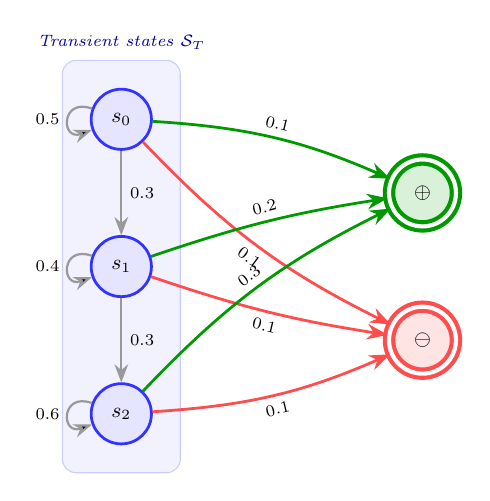
\begin{tikzpicture}[
      >=Stealth,
      scale=0.85, every node/.style={transform shape},
      transient/.style={circle, draw=blue!80, fill=blue!10, line width=1pt, minimum size=0.9cm, font=\small\bfseries},
      absorbing/.style={circle, draw=#1, fill=#1, fill opacity=0.15, text opacity=1, line width=1.5pt, minimum size=1cm, font=\small\bfseries, double, double distance=1.5pt, double=white},
      trans/.style={->, draw=gray!80, line width=0.8pt, font=\scriptsize},
      tosucc/.style={->, draw=green!60!black, line width=1pt, font=\scriptsize},
      tofail/.style={->, draw=red!70, line width=1pt, font=\scriptsize}
  ]
      % States
      \node[transient] (s0) at (0, 2.2)  {$s_0$};
      \node[transient] (s1) at (0, 0)    {$s_1$};
      \node[transient] (s2) at (0,-2.2)  {$s_2$};
      \node[absorbing=green!60!black] (succ) at (4.5, 1.1)  {$\oplus$};
      \node[absorbing=red!70]   (fail) at (4.5,-1.1)  {$\ominus$};

      % Transitions (Q)
      \draw[trans] (s0) edge[loop left, looseness=4, out=160, in=200] node[left] {0.5} (s0);
      \draw[trans] (s0) -- node[right] {0.3} (s1);
      \draw[trans] (s1) edge[loop left, looseness=4, out=160, in=200] node[left] {0.4} (s1);
      \draw[trans] (s1) -- node[right] {0.3} (s2);
      \draw[trans] (s2) edge[loop left, looseness=4, out=160, in=200] node[left] {0.6} (s2);

      % Transitions (R)
      \draw[tosucc] (s0) to[bend left=10]  node[above, sloped] {0.1} (succ);
      \draw[tofail] (s0) to[bend right=10] node[below, sloped] {0.1} (fail);
      \draw[tosucc] (s1) to[bend left=5]   node[above, sloped] {0.2} (succ);
      \draw[tofail] (s1) to[bend right=5]  node[below, sloped] {0.1} (fail);
      \draw[tosucc] (s2) to[bend left=10]  node[above, sloped] {0.3} (succ);
      \draw[tofail] (s2) to[bend right=10] node[below, sloped] {0.1} (fail);

      % Labels
      \begin{scope}[on background layer]
          \node[draw=blue!20, fill=blue!5, rounded corners=5pt, fit=(s0)(s1)(s2), inner sep=10pt] (tbox) {};
      \end{scope}
      \node[text=blue!60!black, font=\scriptsize\itshape, above=1pt of tbox] {Transient states $\mathcal{S}_T$};
  \end{tikzpicture}
  \caption{Illustration of a fitted absorbing DTMC. Transitions among
           transient states (matrix $Q$) model agent logic, while
           success and failure exit vectors $R_\oplus$ and
           $R_\ominus$ lead to absorbing states $\oplus$ and
           $\ominus$.}
  \label{fig:markov_chain}
\end{figure}
\fi
%% ================================================================

\section{State Construction from Traces}
\label{sec:state_construction}

The formalism is useful only if traces can produce the fitted chain
reproducibly and with checks that expose when the abstraction fails. A
fitted Markov model is an estimate plus evidence: the trace
representation, order test, first-passage fit, and uncertainty analysis
must all support its use. Figure~\ref{fig:design} summarizes the
workflow; Algorithm~\ref{alg:trace} implements the construction pipeline
and Algorithm~\ref{alg:gof} the goodness-of-fit (GoF) protocol that SS7
(\S\ref{sec:ss7}) checks on controlled corpora.

%% [REDUCTION] The standalone pipeline figure is superseded by the study-design
%% figure (Fig.~\ref{fig:design}) in \S\ref{sec:intro}. Retained for the artifact.
\iffalse
\begin{figure}[!t]
\centering
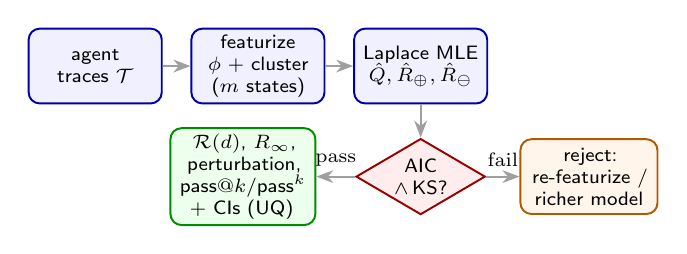
\begin{tikzpicture}[
    >=Stealth, font=\scriptsize\sffamily, node distance=2pt,
    stage/.style={rectangle, rounded corners, draw=blue!65!black, fill=blue!6,
      line width=0.7pt, align=center, text width=1.55cm, minimum height=0.95cm, inner sep=2pt},
    gate/.style={diamond, aspect=1.7, draw=red!60!black, fill=red!7, line width=0.7pt,
      align=center, font=\scriptsize\sffamily, inner sep=1pt},
    result/.style={rectangle, rounded corners, draw=green!55!black, fill=green!7,
      line width=0.7pt, align=center, text width=1.7cm, minimum height=0.95cm, inner sep=2pt},
    ar/.style={->, draw=gray!75, line width=0.7pt}]
  \node[stage] (tr) {agent\\traces $\mathcal T$};
  \node[stage, right=10pt of tr] (fe) {featurize\\$\phi$ + cluster ($m$ states)};
  \node[stage, right=10pt of fe] (mle) {Laplace MLE\\$\hat Q,\hat R_\oplus,\hat R_\ominus$};
  \node[gate, below=12pt of mle] (gof) {AIC\\$\wedge$\,KS?};
  \node[result, left=14pt of gof] (use) {$\mathcal R(d)$, $R_\infty$,\\perturbation,\\pass$@k$/pass$^k$\\+ CIs (UQ)};
  \node[stage, right=12pt of gof, text width=1.6cm, draw=orange!70!black, fill=orange!8] (rej) {reject:\\re-featurize /\\richer model};
  \draw[ar] (tr) -- (fe);
  \draw[ar] (fe) -- (mle);
  \draw[ar] (mle) -- (gof);
  \draw[ar] (gof) -- node[above, font=\scriptsize] {pass} (use);
  \draw[ar] (gof) -- node[above, font=\scriptsize] {fail} (rej);
\end{tikzpicture}
\caption{\textsc{TraceToChain} workflow: traces are featurized and clustered
into $m$ transient states; Laplace-smoothed MLE fits the absorbing chain; the
composite AIC$\,\wedge\,$KS certificate gates whether the first-passage
quantities (with uncertainty) may be reported, or the corpus is referred back
for re-featurization or a richer model.}
\label{fig:pipeline}
\end{figure}
\fi


\subsection{Featurization and Discretization}
\label{sec:featurization}

The first step is to turn heterogeneous trace events into countable
states: reasoning steps, tool calls, and observations are featurized
and then clustered into labels such as ``plan'' or ``tool result.'' Let
$\mathcal{T} = \{\tau^{(i)}\}_{i=1}^{n}$ be the trace corpus. A run is
$\tau^{(i)} = (\sigma_1^{(i)}, \sigma_2^{(i)}, \ldots,
\sigma_{L_i}^{(i)}, y^{(i)})$, where each $\sigma_t^{(i)}$ is one
observed step and $y^{(i)} \in \{\oplus, \ominus\}$ is the terminal
outcome. A featurizer $\phi : \sigma \mapsto \mathbb{R}^p$ maps each
step to a vector representation, either:
\begin{itemize}
  \item \emph{rule-based} (tool type, retry flag, error code, used in
        our simulation study SS7 and MAST experiments), or
  \item \emph{learned} (a pretrained sentence encoder applied to the
        agent's chain-of-thought and interchangeable in
        Algorithm~\ref{alg:trace}).
\end{itemize}
We cluster the feature vectors $\{\phi(\sigma_t^{(i)})\}$ using
agglomerative Ward linkage~\cite{ward1963}. The number of clusters
$m \in [k_{\min}, k_{\max}]$ is selected by silhouette
score~\cite{rousseeuw1987}; we use $[3,6]$ on the controlled corpora of
SS9 and $[2,10]$ on the real corpora, with SS11 varying $k_{\max}$
explicitly. Each step is assigned to the selected
cluster, yielding
$s_1^{(i)}, \ldots, s_{L_i}^{(i)} \in \{1, \ldots, m\}$ followed by
the terminal outcome.

\subsection{Transition Estimation and Order Selection}
\label{sec:order_selection}

Estimating the fitted chain is then a counting problem with a direct
operational reading: a row of $\hat Q$ says where the agent goes next
if it has not terminated, and the matching entries of $\hat R_\oplus$
and $\hat R_\ominus$ say how often that state exits to success or fatal
failure. We fit these quantities by
Laplace-smoothed maximum-likelihood estimation (MLE) with
$\alpha=1$, so
$\hat{Q}_{ij} = (c_{ij} + \alpha) / (c_i + \alpha(m+2))$
where $c_{ij}$ is the count of transitions from state $i$ to state
$j$, $c_{i,\oplus}$ and $c_{i,\ominus}$ count terminal exits from
state $i$, and
$c_i = \sum_j c_{ij} + c_{i,\oplus}+c_{i,\ominus}$. The same
denominator normalizes the success and failure exits. Smoothing
prevents sparse rows from assigning zero probability to unobserved but
plausible exits.

We also test whether first-order memory is sufficient. The comparison
uses a first-vs-second-order Markov Akaike information criterion (AIC)
test~\cite{akaike1974}:
$\Delta_{\rm AIC} = \mathrm{AIC}_1 - \mathrm{AIC}_2
                  = -2(\ell_1 - \ell_2) + 2(k_1 - k_2),$
where $\ell_o$ and $k_o$ are the log-likelihood and free-parameter
count under order $o$. The first-order model is preferred iff
$\Delta_{\rm AIC} < 0$. Simulation study SS7 (\S\ref{sec:ss7}) shows
that this test has high power against second-order ground truth.

\paragraph{Time-homogeneity as a testable assumption.}
When we pool transition counts, we assume a \emph{time-homogeneous}
kernel $\Pr[s_{t+1}=j \mid s_t=i]$ that does not vary with $t$. The
composite AIC$\,\wedge\,$KS protocol (Algorithm~\ref{alg:gof}) tests
whether that simplification is defensible. AIC checks whether recent
history still matters after conditioning on the current state, while
the Kolmogorov--Smirnov (KS) first-passage test can reveal drift in
exit hazards. If either test fails, the corpus should be segmented
before counts are pooled.

\paragraph{Variable horizons, early termination, and censoring.}
Runs can have different lengths and may end in success ($\oplus$),
failure ($\ominus$), or right-censoring. Algorithm~\ref{alg:trace}
counts each observed transient transition once. Completed runs add one
absorber count, while censored runs contribute only the transitions
observed before censoring. This keeps $\hat Q$ tied to observed
movement among transient states, but it can make the exit estimates
$\hat R_\oplus$ and $\hat R_\ominus$ conservative when censoring is
substantial. In \S\ref{sec:mast} we observe censoring below $10\%$, and
SS12 (\S\ref{sec:robustness}) probes far heavier regimes.

\begin{algorithm}[t]
\small
\DontPrintSemicolon
\KwIn{Traces $\mathcal{T}$, featurizer $\phi$, cluster range
      $[k_{\min}, k_{\max}]$, Laplace $\alpha$.}
\KwOut{$\hat{Q}, \hat{R}_\oplus, \hat{R}_\ominus$, labels $\pi$,
       AIC order verdict.}
$X \leftarrow [\phi(\sigma_t^{(i)})]_{i,t}$\tcp*{featurize}
\For{$k = k_{\min}$ \KwTo $k_{\max}$}{
  $L_k \leftarrow$ AgglomerativeWard$(X, k)$;\quad
  $\mathrm{sil}_k \leftarrow $ silhouette$(X, L_k)$\;
}
$m^\star \leftarrow \arg\max_k \mathrm{sil}_k$;\quad
$\pi \leftarrow L_{m^\star}$\;
$c_{s_t,s_{t+1}}\mathrel{+}=1$ for each transient transition;
$c_{s_{L_i},y^{(i)}}\mathrel{+}=1$ for each terminal exit\;
$\hat{Q}_{ij} \leftarrow (c_{ij} + \alpha) / (c_i + \alpha(m^\star + 2))$;
same normalization for $\hat{R}_{\oplus,i},\hat{R}_{\ominus,i}$\;
Compute $\ell_1, \ell_2, k_1, k_2$;\quad
$\Delta_{\rm AIC} \leftarrow -2(\ell_1 - \ell_2) + 2(k_1 - k_2)$\;
\KwRet{$(\hat{Q}, \hat{R}_\oplus, \hat{R}_\ominus, \pi)$;
       first-order iff $\Delta_{\rm AIC} < 0$}\;
\caption{\textsc{TraceToChain}: construct and audit an absorbing DTMC
         from agent execution traces.}
\label{alg:trace}
\end{algorithm}

\subsection{Goodness-of-Fit Protocol}
\label{sec:gof}

Fitting helps only if the abstraction matches the traces. A rejection
is an engineering result, not a nuisance: it says the current state
labels should not be used for reliability queries without segmentation,
new features, or a richer model. We use two checks on $\hat M$ that
address different failure modes:

\emph{Layer 1 (KS on first-passage).} We compare the model
success first-passage-time (FPT) distribution
$F_{\tau_\oplus \mid \tau_\oplus < \tau_\ominus}^{\hat M}$, conditional
on eventual success, with the empirical distribution of success FPTs
among successful traces, and retain the null iff $p_{\rm KS} > 0.05$.
The reference distribution is drawn from $\hat M$ as $N$ seeded
absorption times ($N=8{,}000$ in SS9, $20{,}000$ on the real corpora),
so this is a genuine \emph{two-sample} KS test~\cite{smirnov1939}, not a
one-sample test against a closed-form CDF: stochastic, but
seed-reproducible.

\emph{Layer 2 (AIC).} The AIC layer asks whether the first-order
chain is adequate compared with a second-order alternative. We reject
the first-order model if $\Delta_{\rm AIC} > 0$.

\emph{Composite rule.} The chain is accepted iff
\emph{both} $p_{\rm KS} > 0.05$ \emph{and} $\Delta_{\rm AIC} < 0$.
This rule catches second-order dependence that the FPT-marginal KS test
can miss (see \S\ref{sec:ss7}). If either layer fails, later
reliability quantities should be treated as unsupported by the current
trace abstraction. Given $\phi$, the cluster range, $\alpha$, and a
lowest-$k$ silhouette tie-breaking rule, Algorithm~\ref{alg:trace} is
deterministic in the trace corpus, and Algorithm~\ref{alg:gof} is
deterministic given its reference-sample seed; all seeds are fixed in
the artifact.

\begin{algorithm}[t]
\small
\DontPrintSemicolon
\KwIn{Traces $\mathcal{T}$, fitted chain $\hat{M}$, threshold
      $\alpha_{\rm KS}=0.05$.}
\KwOut{\textsc{Accept} / \textsc{Reject}, $(p_{\rm KS},\Delta_{\rm AIC})$.}
Draw $N$ seeded absorption times from $\hat M$ $\to$ reference
$\tilde F_{\tau_\oplus \mid \tau_\oplus < \tau_\ominus}^{\hat M}$\;
Collect empirical FPTs from $\mathcal{T}_\oplus$ (success traces)\;
$p_{\rm KS} \leftarrow$ two-sample KS($\hat F$, $\tilde F^{\hat M}$)\;
$\Delta_{\rm AIC} \leftarrow$ (Algorithm~\ref{alg:trace}, line~8)\;
\eIf{$p_{\rm KS} > \alpha_{\rm KS}$ \textbf{and} $\Delta_{\rm AIC} < 0$}{
  \KwRet{\textsc{Accept}, $(p_{\rm KS}, \Delta_{\rm AIC})$}\;
}{
  \KwRet{\textsc{Reject}, $(p_{\rm KS}, \Delta_{\rm AIC})$}\;
}
\caption{Composite KS/AIC goodness-of-fit test for the agent-DTMC
         assumption.}
\label{alg:gof}
\end{algorithm}

\subsection{Uncertainty Quantification on \texorpdfstring{$\hat Q$, $\hat R_\oplus$, $\hat R_\ominus$}{Q, R+, R-}}
\label{sec:uq}

Algorithm~\ref{alg:trace} returns point estimates, but a small corpus
may estimate a row of $\hat Q$ or an exit probability poorly, and that
uncertainty should be visible before an operator interprets $R(d)$,
$R_\infty$, or a perturbation result. We therefore attach intervals to
$\hat Q$, $\hat R_\oplus$, and $\hat R_\ominus$ and propagate them to
the quantities of \S\ref{sec:core}--\S\ref{sec:ext}.

\paragraph{(i) Closed-form Dirichlet posterior.}
The Laplace-smoothed MLE is the posterior mean under a symmetric
Dirichlet$(\alpha)$ prior over $\{s_1,\ldots,s_m,\oplus,\ominus\}$. The
row-$i$ posterior is $\mathrm{Dir}(c_{i,\cdot} + \alpha \mathbf{1})$
and the marginal for any single entry $X_{i,j}$ (including absorber
columns) is $\mathrm{Beta}(c_{i,j}+\alpha,\; c_i + \alpha(m+2) -
c_{i,j} - \alpha)$, where $c_i = \sum_{j'} c_{i,j'}$ includes both
transient and absorber outcomes. Equal-tailed $(1-\alpha_{\rm CI})$
credible intervals (CIs) are the corresponding Beta quantiles; we use
$\alpha_{\rm CI}=0.05$ throughout.

\paragraph{(ii) Non-parametric trace-level bootstrap.}
To quantify trace-sampling variability we resample traces with
replacement $B=200$ times, assign each step to its nearest target
centroid to keep labels aligned, and recompute the MLE. The implemented full
re-clustering path (\texttt{fast=False}) gives comparable but wider
intervals.

\paragraph{Empirical ranges.}
Table~\ref{tab:mast-states} reports representative MAST-derived state
taxonomies from SS8; each cluster is named by its dominant rule-based
feature (\S\ref{sec:featurization}) with that feature's within-cluster
share in parentheses, and the posterior intervals show which
success exits are well estimated or sparse, exposing state-level
variation hidden by aggregate pass/fail rates. Across the seven frameworks the two
uncertainty routes agree closely on entries of $\hat Q$: median
posterior CI widths span $0.108$--$0.116$ and median bootstrap widths
$0.084$--$0.103$, while maxima reaching $0.34$ mark the sparse rows. All downstream $\mathcal{R}(d)$, mean time to
absorption ($\mathrm{MTTA}=e_{s_0}^{\top}N\mathbf{1}$), and pass$^k$
quantities inherit these CIs
by propagation (Lipschitz-continuous in $(\hat Q,\hat R_\oplus)$ by
Proposition~\ref{thm:perturb}).

% Auto-generated by SS8_uncertainty_quantification.py
\begin{table}[t]
\centering
\caption{MAST-derived state taxonomy with 95\% posterior success-exit intervals.}
\label{tab:mast-states}
\scriptsize
\setlength{\tabcolsep}{2pt}
\begin{tabular}{l l c c c}
\toprule
\textbf{Framework} & \textbf{Cluster} & \textbf{$\hat{R}_{\oplus,i}$} & \textbf{95\% post.\ CI} & \textbf{$\hat{R}_{\ominus,i}$} \\
\midrule
react~\cite{yao2023react} & tool\_call (100\%) & 0.064 & [0.039,0.094] & 0.067 \\
\tstriped
 & plan (100\%) & 0.076 & [0.048,0.109] & 0.072 \\
 & retry (100\%) & 0.034 & [0.004,0.092] & 0.085 \\
\tstriped
 & reflect (100\%) & 0.081 & [0.038,0.138] & 0.081 \\
 & error\_parse (100\%) & 0.082 & [0.028,0.162] & 0.082 \\
\tstriped
 & wait (100\%) & 0.057 & [0.007,0.153] & 0.057 \\
\midrule
reflexion~\cite{shinn2023reflexion} & plan (100\%) & 0.121 & [0.074,0.178] & 0.027 \\
\tstriped
 & error\_parse (100\%) & 0.083 & [0.041,0.138] & 0.033 \\
 & retry (100\%) & 0.054 & [0.020,0.103] & 0.045 \\
\tstriped
 & reflect (100\%) & 0.104 & [0.056,0.166] & 0.043 \\
 & tool\_call (100\%) & 0.097 & [0.066,0.133] & 0.064 \\
\tstriped
 & wait (100\%) & 0.128 & [0.049,0.236] & 0.064 \\
\bottomrule
\end{tabular}
\end{table}

%% [REDUCTION] tab:uq-summary is a 7x7 grid whose every range is quoted
%% inline below; retained in the artifact.
%% % Auto-generated by SS8_uncertainty_quantification.py
\begin{table}[t]
\centering
\caption{Per-framework 95\% uncertainty widths for entries of $\hat Q$.}
\label{tab:uq-summary}
\scriptsize
\setlength{\tabcolsep}{2pt}
\begin{tabular}{l c c c c c c}
\toprule
 & \multicolumn{3}{c}{\textbf{Posterior CI width}} & \multicolumn{3}{c}{\textbf{Bootstrap CI width}} \\
\cmidrule(lr){2-4}\cmidrule(lr){5-7}
\textbf{Framework} & \textbf{min} & \textbf{median} & \textbf{max} & \textbf{min} & \textbf{median} & \textbf{max} \\
\midrule
react~\cite{yao2023react} & 0.037 & 0.110 & 0.313 & 0.017 & 0.097 & 0.287 \\
\tstriped
reflexion~\cite{shinn2023reflexion} & 0.048 & 0.109 & 0.238 & 0.040 & 0.098 & 0.253 \\
cot\_agent~\cite{wang2024agentsurvey} & 0.029 & 0.111 & 0.337 & 0.008 & 0.084 & 0.288 \\
\tstriped
toolformer~\cite{schick2023toolformer} & 0.041 & 0.108 & 0.241 & 0.034 & 0.101 & 0.208 \\
babyagi~\cite{wang2024agentsurvey} & 0.040 & 0.113 & 0.286 & 0.035 & 0.100 & 0.291 \\
\tstriped
autogpt~\cite{wang2024agentsurvey} & 0.044 & 0.112 & 0.283 & 0.012 & 0.100 & 0.268 \\
agentbench~\cite{agentbench2024} & 0.034 & 0.116 & 0.265 & 0.032 & 0.103 & 0.250 \\
\bottomrule
\end{tabular}
\end{table}


The output is the audited model used for reliability analysis: a
fitted chain plus uncertainty and fit diagnostics. If either layer
rejects, the corpus should be segmented, re-featurized, or treated as
outside the absorbing-DTMC approximation; when both pass, the fitted
chain can be used for reliability queries with the reported intervals.

%% ================================================================

\section{Analytic Tools}
\label{sec:core}

Once a corpus has produced an accepted fitted chain, the question is
what that chain answers without another benchmark run. Three
absorbing-chain tools address the deployment questions of
\S\ref{sec:intro}: reliability at a horizon, sensitivity to a local
change, and compatibility among common benchmark metrics.

\subsection{Closed-Form Reliability}

The first deployment question is reliability under a step budget:
starting at $s_0$, what is the chance of reaching $\oplus$ by step
$d$? In the running loop, this asks whether the agent reaches a
correct final answer within $d$ reasoning/tool/observation steps.

\begin{proposition}[Closed-form reliability; Kemeny--Snell~\cite{kemenysnell}]
\label{thm:closed}
Under Assumptions~\ref{A:trans}--\ref{A:init}, for every
$d\in\mathbb{N}_{\ge 0}$,
\begin{equation}
R(d) = e_{s_0}^\top(I-Q^{d})\,N\,R_\oplus,
\qquad N=(I-Q)^{-1},
\label{eq:t1finite}
\end{equation}
and
$R_\infty = \lim_{d\to\infty}R(d) = e_{s_0}^\top N R_\oplus$.
\end{proposition}

\noindent\emph{Proof idea.}
Summing all paths that spend $t=0,\ldots,d-1$ steps in transient states
and then exit to success gives
$R(d)=e_{s_0}^{\top}\sum_{t=0}^{d-1}Q^tR_\oplus$; the identity
$\sum_{t=0}^{d-1}Q^t=(I-Q^d)(I-Q)^{-1}$ yields \eqref{eq:t1finite}, and
transience gives $Q^d\to0$. Since $N_{ij}$ is the expected number of
visits to state $j$ before absorption, the closed form separates two
effects an operator can inspect: how often the agent visits each state,
and how likely success is after those visits.

\subsection{Perturbation Sensitivity}

The second question is counterfactual: if a local transition changes,
how much can end-to-end reliability move? A new fallback tool may
change one row of $Q$ by redirecting failed tool calls back to
planning, and the fitted chain gives a first-order sensitivity
calculation before any benchmark rerun.

\begin{proposition}[Perturbation sensitivity; Stewart~\cite{stewart1998}]
\label{thm:perturb}
Let $Q(\varepsilon)=Q_0+\varepsilon\Delta$ be the perturbation family
from Definition~\ref{def:perturb}. Write
$N_0=(I-Q_0)^{-1}$ and let $R_{\oplus,0}$ be the fixed success-exit
vector. Assume
$\varepsilon_{\max}\|N_0\|_\infty\|\Delta\|_\infty<1$.
For every $0\le\varepsilon\le\varepsilon_{\max}$,
\begin{equation}
\bigl|R_\infty(\varepsilon)-R_\infty(0)\bigr|
\le
\varepsilon \|N_0\|_\infty^2\|\Delta\|_\infty
        \|R_{\oplus,0}\|_\infty
 + C\varepsilon^2,
\label{eq:t2}
\end{equation}
with
$C=\|N_0\|_\infty^3\|\Delta\|_\infty^2\|R_{\oplus,0}\|_\infty
 /(1-\varepsilon_{\max}\|N_0\|_\infty\|\Delta\|_\infty)$. Moreover,
\begin{equation}
R_\infty(\varepsilon)-R_\infty(0)
=\varepsilon e_{s_0}^{\top}N_0\Delta N_0R_{\oplus,0}
 + O(\varepsilon^2).
\label{eq:t2lin}
\end{equation}
\end{proposition}

\noindent\emph{Proof idea.}
Expand $(I-Q(\varepsilon))^{-1}$ with the Neumann series around $Q_0$;
the smallness condition bounds the remainder by the displayed constant.
In the first-order term $N_0\Delta N_0$, the left factor counts how
often execution reaches the changed row and the right factor measures
success value after the perturbed transition, so a large
$\|N_0\|_\infty$ warns that small local changes can have large global
effects. The bound is best read as a screening calculation that
identifies local changes meriting a new benchmark run. As stated it
applies to perturbations of $Q$ with $R_\oplus$ fixed; changes to
success exits require the corresponding linear term for the exit
vector, and the real-data fallback-tool result of \S\ref{sec:ss14} is
of that second kind, so we evaluate it exactly from
Proposition~\ref{thm:closed} rather than through this bound.

\subsection{Metric Unification}
\label{sec:unify}

The third question is semantic. pass$@k$, pass$^k$, and the RDC often
appear to be competing summaries, but under the fitted chain they are
different views of one first-passage distribution: the disagreement is
about which projection to report, not about the underlying reliability
event. We keep the benchmark name RDC, but the quantity modeled here is
the cumulative success probability by horizon $d$.

\begin{theorem}[Metric unification]
\label{thm:unify}
Let $R_\infty=e_{s_0}^{\top}NR_\oplus$. Under the i.i.d.\
replication assumption A\ref{A:iid},
\begin{align}
\mathrm{pass}^{k} &= R_\infty^{k}, \label{eq:t3-passk}\\
\mathrm{pass}@k  &= 1-(1-R_\infty)^{k}, \label{eq:t3-passatk}\\
\mathrm{RDC}(d)  &= R(d)
 = e_{s_0}^{\top}(I-Q^{d})NR_\oplus. \label{eq:t3-rdc}
\end{align}
Thus the three metrics are restrictions or transformations of the
same first-passage distribution.
\end{theorem}

\noindent\emph{Proof idea.}
pass$^k$ is the probability that all $k$ independent trials succeed,
pass$@k$ is one minus the probability that all $k$ fail, and the RDC is
the finite-horizon reliability of Proposition~\ref{thm:closed}.

Repeated agent runs can, however, share latent conditions such as a
common prompt template, cache state, or task difficulty. The next
result makes that caveat measurable: it shows how shared variation
changes the two repeated-trial metrics even when marginal reliability
remains $R_\infty$.

\begin{theorem}[Correlated-trial inequalities]
\label{thm:corr}
Suppose the $k$ trials share a latent state $\xi$ with
$\Pr[X_i=1\mid\xi]=p(\xi)$ and
$\mathbb{E}_\xi[p(\xi)]=R_\infty$, and are independent conditional on
$\xi$. Then
\begin{align}
\mathrm{pass}^{k} &= \mathbb{E}_\xi[p(\xi)^k]
                  \ge R_\infty^k, \label{eq:t3p-passk}\\
\mathrm{pass}@k  &= 1-\mathbb{E}_\xi[(1-p(\xi))^k]
                  \le 1-(1-R_\infty)^k. \label{eq:t3p-passatk}
\end{align}
For $k\ge2$, equality holds iff $p(\xi)$ is almost surely constant.
\end{theorem}

\noindent\emph{Proof idea.}
Condition on the latent variable and apply Jensen's inequality to
the convex functions $p^k$ and $(1-p)^k$.

\begin{corollary}[Diagnostic]
\label{cor:diag}
The gap
$\widehat{\mathrm{pass}^{k}}-\hat R_\infty^{\,k}$ is a
lightweight diagnostic for hidden cross-trial correlation. Large
positive gaps indicate that repeated trials are not behaving as
i.i.d.\ samples from one fixed chain.
\end{corollary}

Hidden heterogeneity thus raises all-success estimates and lowers
at-least-one-success estimates relative to the i.i.d.\ formulas, so a
large gap should trigger inspection before repeated samples are treated
as independent trials: an assumption behind pass$@k$ and pass$^k$
becomes a diagnostic rather than a hidden convention.

\section{Extensions}
\label{sec:ext}

Three extensions help interpret those answers: why an RDC may
saturate, when a classical reliability-growth curve emerges, and how
many steps are needed before $R(d)$ approaches $R_\infty$.

\subsection{RDC Shape}

An RDC is more useful when its shape has an explanation: a concave
curve suggests early steps resolve the easier cases while later ones
add less, and a convex window suggests a barrier such as waiting on a
tool response. The following condition captures the common
early-gains/saturation pattern.

\begin{assumption}[Stochastic monotonicity of $Q$]\label{A:monotone}
Fix an order $\preceq$ on the transient states. The matrix $Q$ is
\emph{stochastically monotone} if $Qf$ is non-increasing whenever
$f:\ST\to\mathbb{R}_{\ge0}$ is; equivalently, later rows of $Q$ place
stochastically more mass on later states in the
order~\cite{daley1968stochastic,karlin1968tp,keilsonKester1977}.
\end{assumption}

\begin{proposition}[RDC shape; Keilson--Kester~\cite{keilsonKester1977},
Karlin--Rinott~\cite{karlin1980tp2}]
\label{thm:shape}
Let $v=e_{s_0}^{\top}$ and $w=R_\oplus$. For
$R(d)=v(I-Q^d)NR_\oplus$,
\begin{equation}
\Delta R(d)=R(d+1)-R(d)=vQ^dw\ge0,
\label{eq:t4-1stdiff}
\end{equation}
and, for $d\ge1$,
\begin{equation}
\Delta^2R(d)=R(d+1)-2R(d)+R(d-1)
           =-vQ^{d-1}(I-Q)w.
\label{eq:t4-2nddiff}
\end{equation}
If $Qw\le w$ componentwise, then $R(d)$ is globally concave.
Assumption~\ref{A:monotone} together with $w$ non-increasing in the
state order is the structural regime in which that dominance is
expected; the concavity conclusion itself needs only $Qw\le w$.
\end{proposition}

\noindent\emph{Proof idea.}
The first difference is the probability of exiting to success exactly
after $d$ transient steps, so reliability never decreases with more
steps; since $vQ^{d-1}\ge0$, \eqref{eq:t4-2nddiff} makes $Qw\le w$
sufficient for a nonpositive second difference. A convex empirical
window instead signals an early barrier.

\subsection{NHPP Rare-Failure Limit}

The absorbing-chain view also explains when aggregate
reliability-growth curves emerge from step-level behavior---not as a
separate modeling story but as the rare-failure limiting case in which
a one-state chain reduces to Goel--Okumoto.

\begin{proposition}[NHPP rare-failure limit; Goel--Okumoto~\cite{goelokt}]
\label{thm:nhpp}
Consider a sequence of one-transient-state agent chains with per-step
success probability $\mu_n$, per-step failure probability
$\varepsilon_n$, and $Q_n=1-\mu_n-\varepsilon_n$. Suppose
$\mu_n\to0$, $\varepsilon_n\to0$, $d_n\mu_n\to\Lambda\in(0,\infty)$,
and $\varepsilon_n/\mu_n\to0$. For any fixed $c>0$ and $d=cd_n$, the
cumulative first-passage CDF converges to
\begin{equation}
R_n(d)\to 1-e^{-c\Lambda},
\label{eq:t5-GO}
\end{equation}
the Goel--Okumoto NHPP mean-value form $m(t)=a(1-e^{-bt})$ with
normalized $a=1$.
\end{proposition}

\noindent\emph{Proof idea.}
For the one-state chain,
$R_n(d)=\frac{\mu_n}{\mu_n+\varepsilon_n}
\left(1-(1-\mu_n-\varepsilon_n)^d\right)$. Under rare-failure
scaling the prefactor tends to one and the geometric term tends to
$e^{-c\Lambda}$. Outside this low-error regime, the exact closed form
of Proposition~\ref{thm:closed} should be used.

\subsection{Approach-Rate Bound}

Even when $R_\infty$ is known, a practitioner still needs a step
budget. The next result converts spectral decay of $Q$ into a
conservative horizon rule: how many more agent steps are needed before
the remaining reliability gap is at most $\delta$?

\begin{proposition}[Approach-rate bound; Horn--Johnson~\cite{hornjohnson2013},
Stewart~\cite{stewart1998}, Levin--Peres~\cite{levin2017markov}]
\label{thm:mixing}
Let $\rho=\rho(Q)<1$ and $N=(I-Q)^{-1}$. If
$Q=V\Lambda V^{-1}$ is diagonalizable, then
$R_\infty-R(d)\le\kappa_\infty(V)\rho^d\|NR_\oplus\|_\infty$
with $\kappa_\infty(V)=\|V\|_\infty\|V^{-1}\|_\infty$, so a
sufficient horizon for error at most $\delta$ is
\begin{equation}
d^\star_{\mathrm{diag}}(\delta)=
\max\!\left\{0,\left\lceil
\frac{\log(\kappa_\infty(V)\|NR_\oplus\|_\infty/\delta)}
     {-\log\rho}
\right\rceil\right\}.
\label{eq:t6-steps-diag}
\end{equation}
For non-diagonalizable $Q$, the same exponential term is multiplied
by a polynomial factor determined by the largest Jordan block.
\end{proposition}

\noindent\emph{Proof idea.}
The gap is $R_\infty-R(d)=e_{s_0}^{\top}Q^dNR_\oplus$, so bounding it
reduces to bounding $\|Q^d\|$; diagonalization gives
$\|Q^d\|_\infty\le\kappa_\infty(V)\rho^d$ and Jordan blocks add a
polynomial multiplier, so large $\rho(Q)$ or ill-conditioned
eigenvectors imply longer step budgets. Together these results connect
finite-horizon reliability, classical reliability growth, and
conservative step budgets within one fitted-chain view.

%% ================================================================

\section{Simulation Validation}
\label{sec:sim}

We keep the artifact's study numbering, so the theorem-backing
simulations SS2--SS5 are reported there. The controlled checks below do
not validate unseen operational traces; they show that the computation,
analytic claims, and diagnostics behave as intended on controlled
inputs.

\subsection{SS1 and the Analytic Checks}

SS1 isolates the numerical calculation behind the reliability estimates.
We generate 500 random substochastic chains per size
$m \in \{5, 10, 50, 100, 500\}$ and compare $R_\infty$
(Proposition~\ref{thm:closed}) with Monte Carlo estimates from $10^5$
trajectories per chain, used as an independent simulation baseline for
the same fitted chain rather than as a competing estimator. The absolute
error $|R_\infty^{\rm cf} - \hat R_\infty^{\rm MC}|$ stays below the
$5\%$ acceptance threshold at every size, which supports the closed-form
computations used later in SS6 and SS9 while leaving the Markov-fit
question to the GoF protocol.

Three further controlled checks, reported in full in the artifact,
confirm the analytic claims. The perturbation bound of
Proposition~\ref{thm:perturb} tracks the true
$|R_\infty(\varepsilon)-R_\infty(0)|$ over $\varepsilon\in[0,0.28]$, so
it screens local changes by direction and scale before a full rerun. The
correlated-trial gap of Theorem~\ref{thm:corr} grows with $k$ and with
$\mathrm{Var}(p(\xi))$, confirming that agreement, pass$^k$, and the
independent-trial calculation are different projections of first-passage
behavior rather than interchangeable scalars. Finally, across six
rare-failure scaling regimes the cumulative first-passage curve
converges to the Goel--Okumoto mean-value form
(Proposition~\ref{thm:nhpp}), so Goel--Okumoto appears as a limiting case
of the agent-chain model rather than an unrelated baseline.

%% ----------------------------------------------------------------
%% [REDUCTION] SS2--SS5 (theorem-backing simulations) and the
%% figures fig_ss1_cf_vs_mc / fig_perturbation / fig_correlation_gap /
%% fig_nhpp_limit are suppressed from the 12-page body. They are
%% retained in source and in the reproducibility artifact (see
%% code/sim/SS1*--SS5*.py and figs/). The body retains SS1 as a basic
%% closed-form sanity check and SS7 (goodness-of-fit protocol
%% validation) as the statistical foundation for SS9.
%% ----------------------------------------------------------------
\iffalse
\begin{figure}[!t]
  \centering
  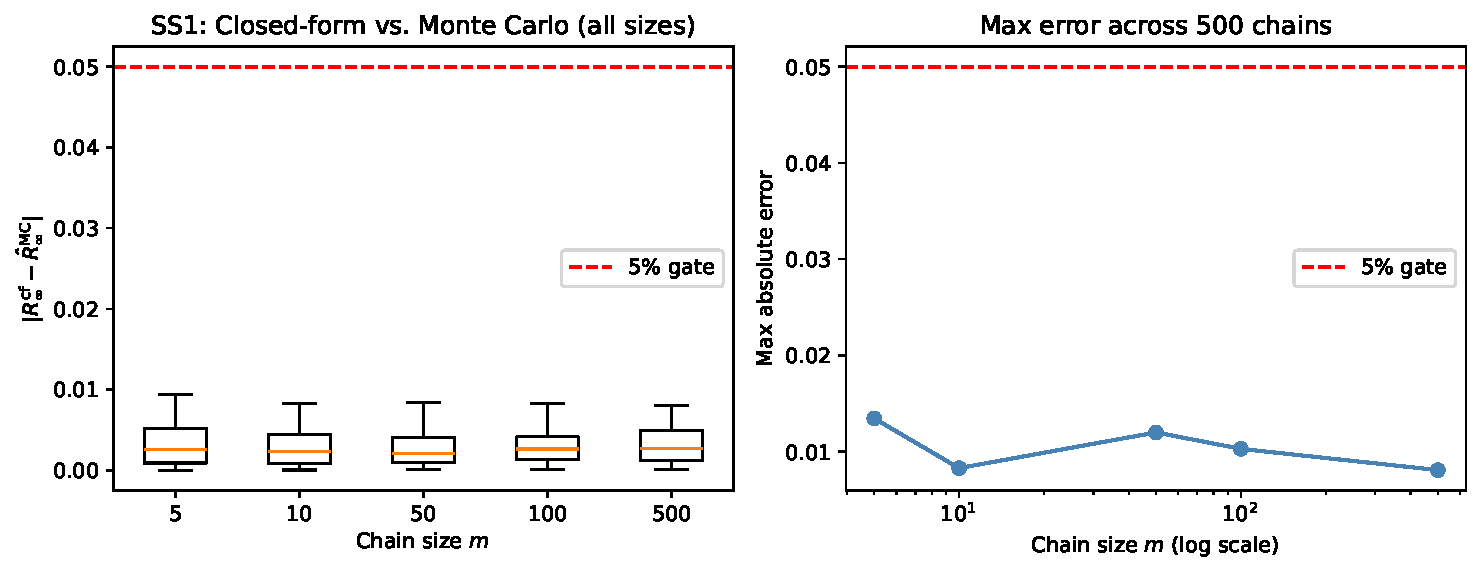
\includegraphics[width=\columnwidth]{../figs/fig_ss1_cf_vs_mc.pdf}
  \caption{SS1 closed-form validation: absolute error
           $|R_\infty^{\rm cf} - \hat{R}_\infty^{\rm MC}|$ between
           analytic eventual-success reliability and Monte Carlo
           estimates across 500 chains per size. All errors are below
           the 5\% G2 threshold.}
  \label{fig:ss1}
\end{figure}

\begin{figure}[!t]
  \centering
  \begin{minipage}[t]{0.32\columnwidth}
    \centering
    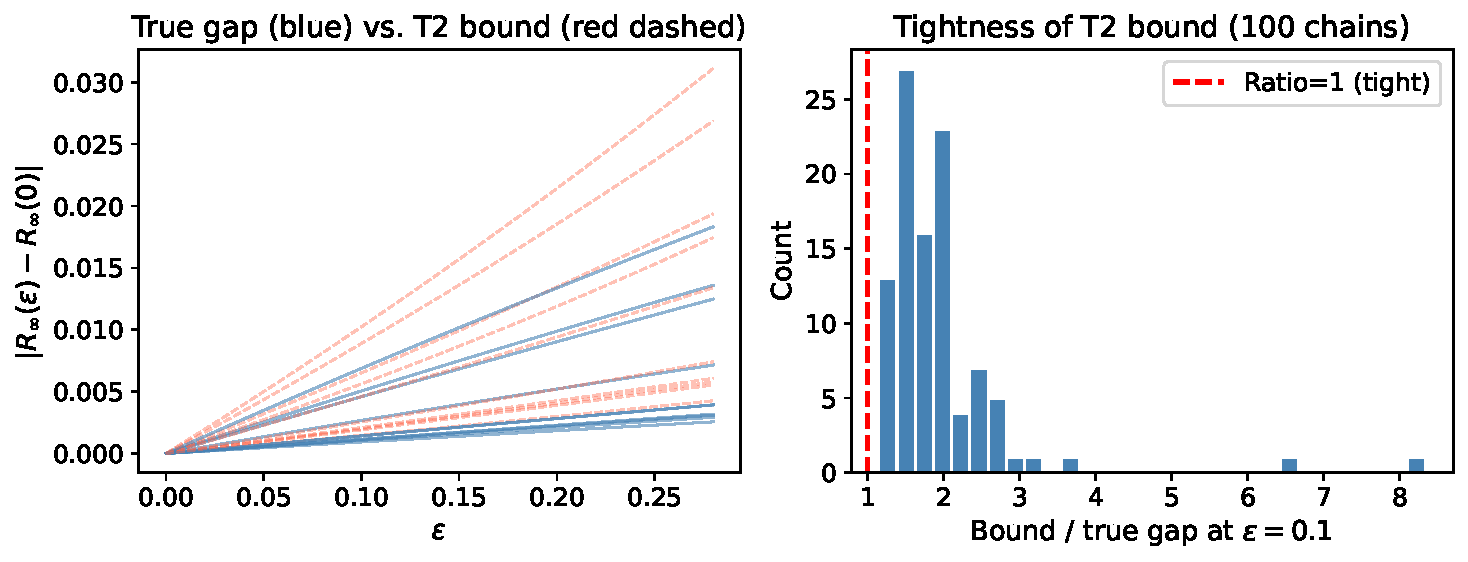
\includegraphics[trim=0bp 0bp 350bp 0bp,clip,width=\linewidth,height=0.075\textheight,keepaspectratio]{../figs/fig_perturbation.pdf}\\[-0.3ex]
    {\scriptsize (a) Perturbation}
  \end{minipage}\hfill
  \begin{minipage}[t]{0.32\columnwidth}
    \centering
    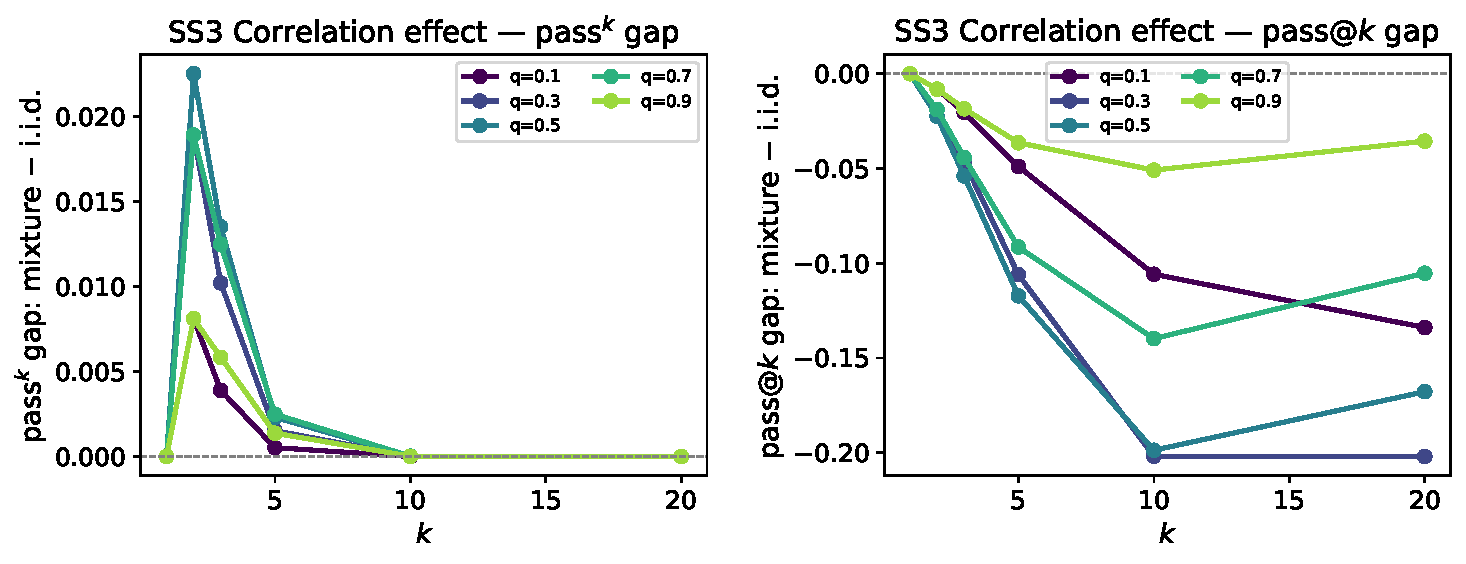
\includegraphics[trim=0bp 0bp 365bp 0bp,clip,width=\linewidth,height=0.075\textheight,keepaspectratio]{../figs/fig_correlation_gap.pdf}\\[-0.3ex]
    {\scriptsize (b) Agreement}
  \end{minipage}\hfill
  \begin{minipage}[t]{0.32\columnwidth}
    \centering
    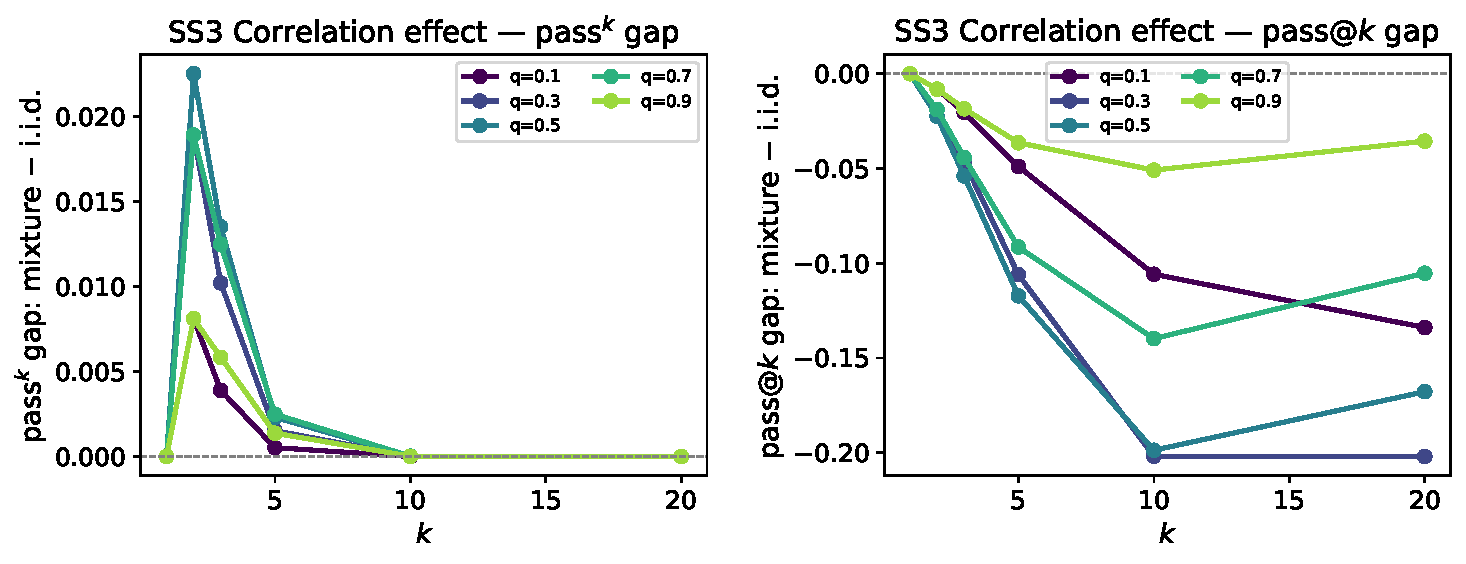
\includegraphics[trim=365bp 0bp 0bp 0bp,clip,width=\linewidth,height=0.075\textheight,keepaspectratio]{../figs/fig_correlation_gap.pdf}\\[-0.3ex]
    {\scriptsize (c) pass$^k$}
  \end{minipage}
  \caption{Additional theorem checks retained in the artifact:
           (a) perturbation bound behavior, (b) correlated-trial
           agreement lift, and (c) pass$^k$ gap.}
  \label{fig:analytic_checks}
\end{figure}

\begin{figure}[!t]
  \centering
  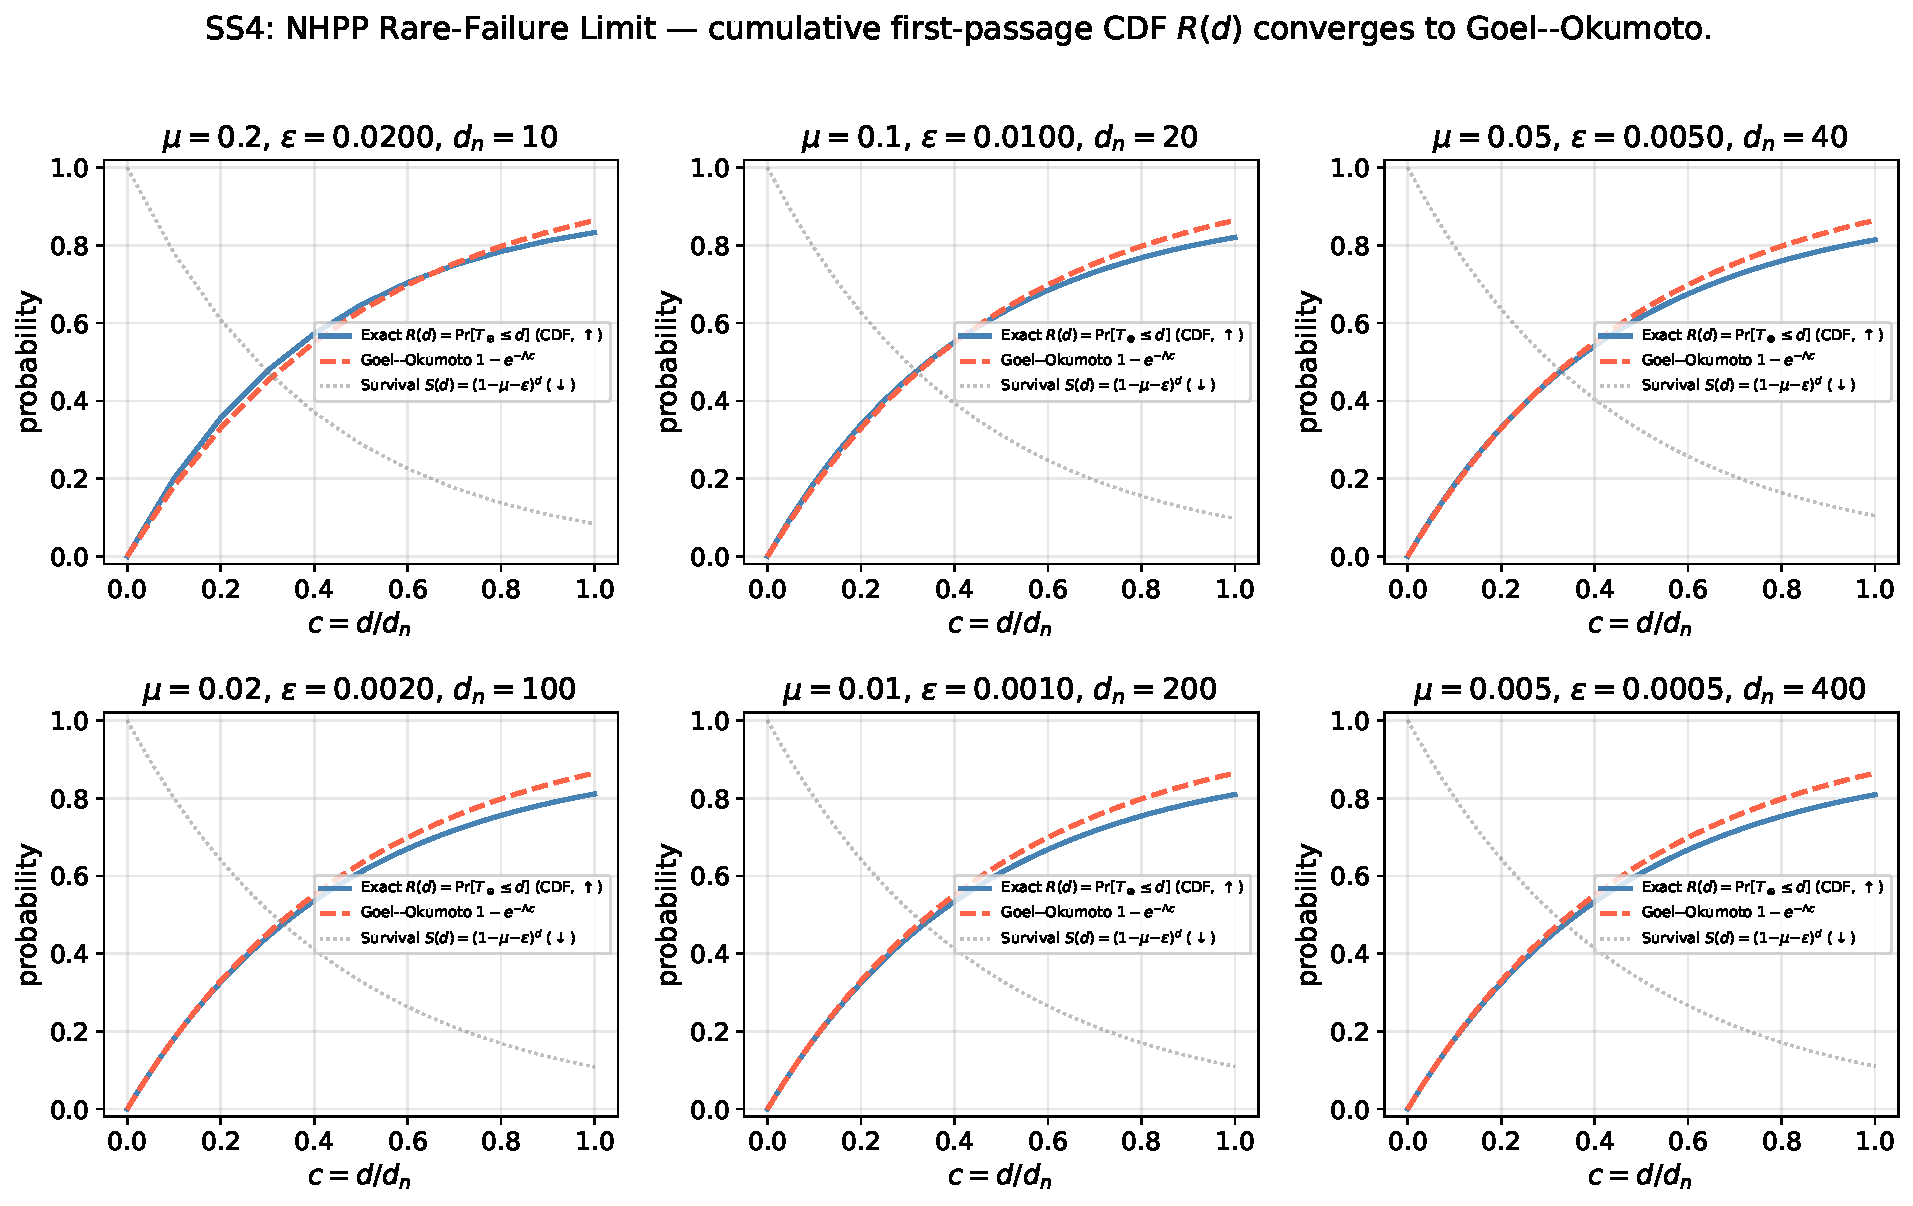
\includegraphics[width=\columnwidth,height=0.16\textheight,keepaspectratio]{../figs/fig_nhpp_limit.pdf}
  \caption{Goel--Okumoto rare-failure limit check: the cumulative
           first-passage distribution of the fitted-chain model
           approaches the NHPP mean-value form across six scaling
           regimes.}
  \label{fig:goel_okumoto_limit}
\end{figure}

\subsection{SS2: Perturbation Bound Tightness}

For 100 chains ($m=10$), we sweep $\varepsilon \in [0, 0.28]$ and compare
the T2 analytic bound against the true $|R_\infty(\varepsilon) -
R_\infty(0)|$.

\subsection{SS3: Correlation Effect on pass$^k$}

The gap $\mathrm{pass}^k_{\rm mix} - R_\infty^k$ as a function of $k$ and
mixing probability $q$ confirms the Jensen inequality in
Theorem~\ref{thm:corr}.

\subsection{SS4: NHPP Limit Verification}

We generate a sequence of 1-state agent chains with per-step success
rate $\mu_n\in\{0.2, 0.1, 0.05, 0.02, 0.01, 0.005\}$, per-step failure
rate $\varepsilon_n = 0.1\,\mu_n$, and horizon $d_n = \lceil
\Lambda/\mu_n\rceil$ with $\Lambda=2.0$. For each $n$ we compare the
\emph{cumulative first-passage CDF}
$R_n(d)=\mu_n/(\mu_n+\varepsilon_n)\cdot(1-(1-\mu_n-\varepsilon_n)^d)$
against the Goel--Okumoto mean-value function $1-e^{-\Lambda c}$ in the
rescaled horizon $c=d/d_n$. The KS distance between the two CDFs is
monotone non-increasing in $n$ and the asymptotic $p$-value exceeds
$0.05$ for all six scaling points, confirming
Proposition~\ref{thm:nhpp}. The \emph{survival} function
$S_n(d)=(1-\mu_n-\varepsilon_n)^d$ is separate from $R(d)$ and is not
what Goel--Okumoto predicts.

\subsection{SS5: PRISM Cross-Check}

We export 5 chains ($m=5$) to PRISM DTMC format and run the
query \texttt{P=? [F<=20 "success"]}.  Python closed-form matches PRISM
results to within $10^{-8}$, confirming bit-for-bit correctness.
\fi
%% [END REDUCTION — SS1/SS2/SS3/SS4/SS5 figures]

\subsection{SS7: Goodness-of-Fit of the Agent-DTMC Assumption}
\label{sec:ss7}

SS7 tests the goodness-of-fit protocol of \S\ref{sec:gof}
(Algorithm~\ref{alg:gof}) on three controlled conditions. The goal is
not to make every trace Markov, but to separate corpora where the
fitted-chain abstraction is credible from those where it is not.

\emph{(A) Markov ground truth.} On $30$ corpora of $300$ traces from a
known 1st-order absorbing chain ($m=5$), the composite test retains the
null in $100\%$ of corpora at $\alpha=0.05$; since a nominal $5\%$ test
would reject once or twice in $30$ replicates, the observed size is
\emph{conservative} rather than exactly nominal.
\emph{(B) 2nd-order ground truth.} On $15$ corpora from a 2nd-order
chain with mixture weight $0.6$, the FPT-KS layer alone rejects $0\%$
while the AIC layer rejects $100\%$ with
$\Delta_{\rm AIC}\in[+979,+1614]$, so the composite
accept-if-both-pass rule rejects $100\%$.
\emph{(C) MAST-derived self-consistency.} Sampling 500 synthetic traces
from each of the 7 MAST-derived chains of \S\ref{sec:mast}, the
composite test accepts all 7 (KS $p$-values
$\in\{0.320, 0.374, 0.541, 0.828, 0.910, 0.994, 1.000\}$, with the AIC
layer preferring the first-order model in every case). Because these
traces are sampled from the fitted chain, (C) checks internal
consistency, not whether real agent traces are Markov; the held-out
study next checks whether the full pipeline recovers first-passage
behavior on controlled MAST-style traces it did not fit.

%% [REDUCTION] fig:gof is suppressed for the 12-page body: conditions (A)--(C) above report
%% every number it plots. Retained in the artifact (figs/fig_gof.pdf).
\iffalse
\begin{figure}[!t]
  \centering
  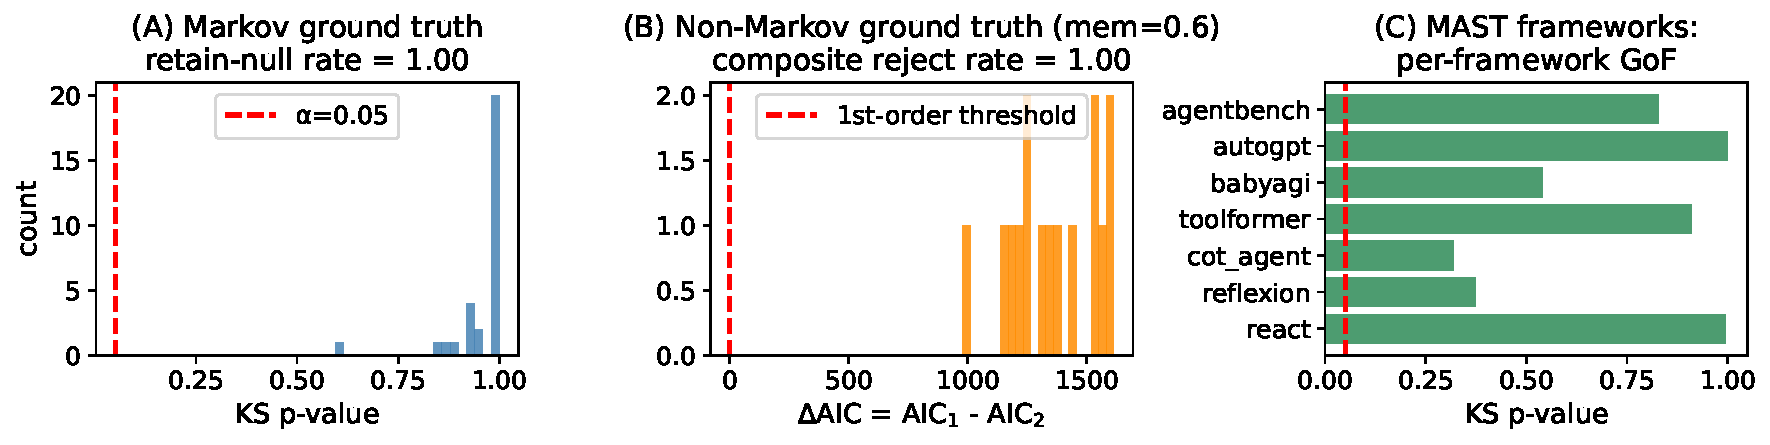
\includegraphics[width=\columnwidth]{../figs/fig_gof.pdf}
  \\[-0.3ex]
  \begin{minipage}[t]{0.32\columnwidth}
    \centering
    {\scriptsize (a) Markov ground truth: KS $p$-values}
  \end{minipage}\hfill
  \begin{minipage}[t]{0.32\columnwidth}
    \centering
    {\scriptsize (b) 2nd-order ground truth: AIC rejection}
  \end{minipage}\hfill
  \begin{minipage}[t]{0.32\columnwidth}
    \centering
    {\scriptsize (c) MAST-derived: self-consistency KS}
  \end{minipage}
  \caption{SS7 tests the GoF safeguard across Markov ground truth,
           2nd-order ground truth, and MAST-derived self-consistency
           conditions.}
  \label{fig:gof}
\end{figure}
\fi


SS1, the artifact checks of
Propositions~\ref{thm:perturb} and~\ref{thm:nhpp} and
Theorem~\ref{thm:corr}, and SS7 thus form a validation ladder that separates numerical correctness, analytic
behavior, and diagnostic behavior from the held-out recovery tested
next.

%% ================================================================

\section{Empirical Case Studies}
\label{sec:case_studies}

The empirical evidence serves two purposes: SS6 illustrates the
reliability quantities on MAST-derived framework summaries, while SS9
uses a strict held-out split to test whether \textsc{TraceToChain}
recovers the RDC and success-time distribution on unseen traces.

\subsection{MAST Benchmark Formulation}
\label{sec:mast}

SS6 uses transition matrices derived from public MAST summaries for
seven frameworks, applies the fitted-chain quantities, and ranks
frameworks by $R_\infty$. The exercise is illustrative: it does not
claim that raw MAST traces are Markov, but it shows what the reliability
vocabulary reports once a chain is available. Asymptotic reliability
spans $R_\infty\in[0.058,0.450]$: it is highest for
toolformer~\cite{schick2023toolformer} and lowest
($\le\!0.07$) for react~\cite{yao2023react}, cot\_agent, and
reflexion~\cite{shinn2023reflexion}, over
$m\in[5,12]$ states with $\rho(Q)\in[0.37,0.66]$ and $\delta{=}0.01$
horizons of $3$--$9$ steps. The full table and the corresponding decay
curves are in the artifact.

%% [REDUCTION] The illustrative SS6 table is suppressed for the 12-page body;
%% its range is quoted inline above and the full table is in the artifact.
\iffalse
\begin{table}[!t]
\centering
\caption{Closed-Form Reliability of MAST Frameworks.}
\label{tab:mast}
\begin{tabular}{lrrrr}
\toprule
\textbf{Framework} & \textbf{$R_\infty$} & \textbf{$\rho(Q)$} & \textbf{Horizon ($\delta=0.01$)} & \textbf{$m$} \\
\midrule
\thighlight
toolformer~\cite{schick2023toolformer}  & 0.4497 & 0.442 &  5 & 10 \\
\tstriped
autogpt~\cite{wang2024agentsurvey}     & 0.3866 & 0.370 &  4 &  5 \\
agentbench~\cite{agentbench2024}  & 0.3262 & 0.654 &  9 & 10 \\
\tstriped
babyagi~\cite{wang2024agentsurvey}     & 0.2853 & 0.656 &  8 & 12 \\
reflexion~\cite{shinn2023reflexion}   & 0.0695 & 0.636 &  5 & 12 \\
\tstriped
cot\_agent~\cite{wang2024agentsurvey}  & 0.0684 & 0.526 &  3 & 10 \\
react~\cite{yao2023react}       & 0.0581 & 0.509 &  3 &  9 \\
\bottomrule
\end{tabular}
\end{table}
\fi


\subsection{SS9: Held-Out Empirical Validation}
\label{sec:ss9}

SS7(C) is an in-sample self-consistency check; SS9 instead evaluates
controlled held-out recovery with a strict fit/test protocol. The test
set is not used to choose features, clusters, transition estimates, or
tuning, so the reported KS and RDC errors measure held-out recovery
rather than reuse of the training corpus.

\paragraph{Protocol.}
For each of the 7 MAST-style frameworks we generate $n=400$
trajectories from a ground-truth absorbing chain whose transient
structure mimics the MAST taxonomy and emits noisy one-hot features
(Gaussian noise $\sigma=0.08$ and $\approx\!5\%$ censored traces). The
corpus is split \emph{before} featurization into
$n_{\mathrm{fit}}=200$ and $n_{\mathrm{test}}=200$. We run
\textsc{TraceToChain} on the fit half only.

Table~\ref{tab:heldout-ss9} reports the recovered state count $m$, the KS
agreement between the model success-time cumulative distribution
function (CDF)
$F_{\tau_\oplus \mid \tau_\oplus < \tau_\ominus}^{\hat M}$,
conditional on eventual success and sampled with $N{=}8{,}000$
trajectories, and the held-out success-time CDF
$\hat F_{\tau_\oplus}$ among successful traces. The table also reports
the sup-norm discrepancy
$L_\infty^{\mathrm{RDC}} =
\sup_{d\in[0,50]} |\mathcal R(d;\hat M) - \hat{\mathcal R}_{\mathrm{emp}}(d)|$.
These are all first-passage checks: they ask whether the fitted chain
predicts \emph{when} success occurs on traces it did not fit. The
held-out empirical RDC is the non-parametric baseline over observed
horizons; the fitted chain is useful only when it tracks that curve and
passes GoF, and it then adds state-level interpretation, uncertainty
propagation, perturbation analysis, metric reconciliation, and horizon
queries beyond the observed grid.

% Auto-generated by SS9_heldout_empirical.py
\begin{table}[t]
\centering
\caption{SS9: held-out recovery on seven controlled MAST-style corpora.}
\label{tab:heldout-ss9}
\small
\begin{tabular}{l c c c c c c}
\toprule
\textbf{Framework} & \textbf{$n_{\mathrm{fit}}$} & \textbf{$n_{\mathrm{test}}$} & \textbf{$m$} & \textbf{$D_{\mathrm{KS}}$} & \textbf{$p_{\mathrm{KS}}$} & \textbf{$L_\infty^{\mathrm{RDC}}$} \\
\midrule
react~\cite{yao2023react} & 200 & 200 & 5 & 0.020 & 1.000 & 0.048 \\
\tstriped
reflexion~\cite{shinn2023reflexion} & 200 & 200 & 5 & 0.033 & 0.984 & 0.052 \\
cot\_agent~\cite{wang2024agentsurvey} & 200 & 200 & 5 & 0.023 & 1.000 & 0.018 \\
\tstriped
toolformer~\cite{schick2023toolformer} & 200 & 200 & 5 & 0.030 & 0.994 & 0.052 \\
babyagi~\cite{wang2024agentsurvey} & 200 & 200 & 6 & 0.045 & 0.827 & 0.053 \\
\tstriped
autogpt~\cite{wang2024agentsurvey} & 200 & 200 & 6 & 0.036 & 0.960 & 0.039 \\
agentbench~\cite{agentbench2024} & 200 & 200 & 5 & 0.030 & 0.995 & 0.021 \\
\bottomrule
\end{tabular}
\end{table}


\begin{figure}[!t]
  \centering
  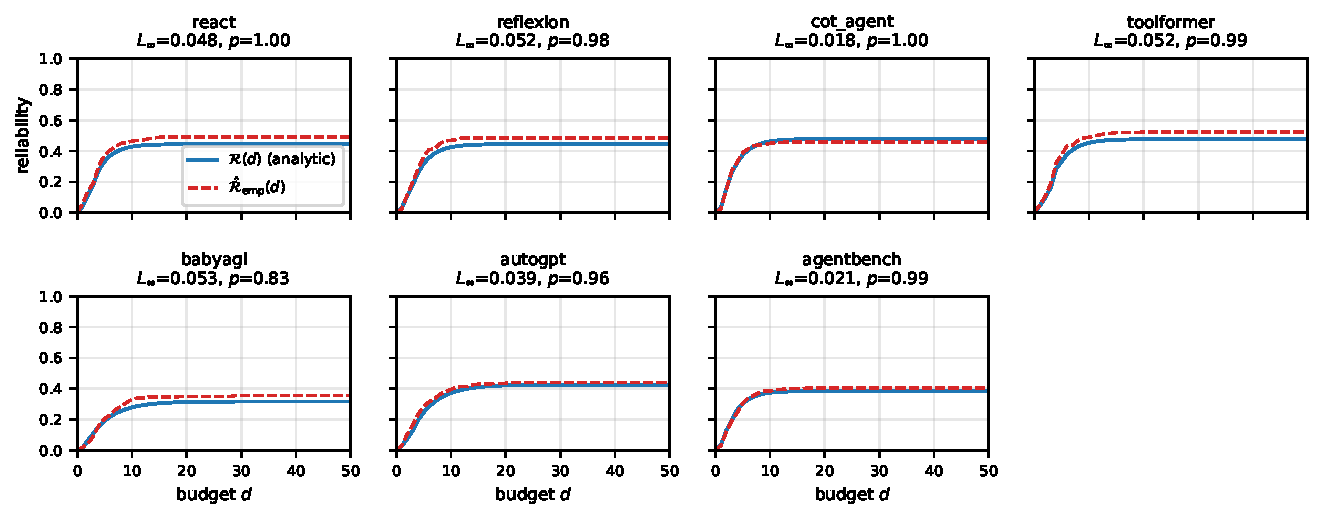
\includegraphics[width=\columnwidth]{../figs/fig_rdc_overlay.pdf}
  \caption{SS9: held-out empirical RDC over the analytic $\mathcal R(d)$.}
  \label{fig:rdc_overlay}
\end{figure}

\paragraph{Findings.}
Figure~\ref{fig:rdc_overlay} overlays, for each framework, the held-out
empirical RDC $\hat{\mathcal R}_{\mathrm{emp}}(d)$ (dashed) on the
analytic $\mathcal R(d)$ of the fitted chain (solid), with each panel
title reporting that framework's $L_\infty^{\mathrm{RDC}}$ and
$p_{\mathrm{KS}}$. The two curves track each other over the whole budget range
$d\in[0,50]$---worst case $0.053$ on babyagi---including the saturation
elbow that the closed form must reproduce to answer horizon queries. Across
all 7 frameworks, the composite diagnostic passes on held-out data at
$\alpha=0.05$. KS distances are small
($D_{\mathrm{KS}}\in[0.020,0.045]$), the minimum KS $p$-value is
$0.827$, and $\max L_\infty^{\mathrm{RDC}}=0.053$ with median $0.048$.
BabyAGI has the largest RDC discrepancy yet still passes KS. This
supports recovery of the success first-passage distribution and RDC
for these controlled MAST-style traces.

\paragraph{Scope.}
SS9 uses synthetic traces from a genuine absorbing chain with noisy
emissions, so the held-out KS test probes controlled recovery by the
trace-to-chain pipeline:
featurization, clustering, Markov-order testing, and MLE. It does not
prove that operational agent traces are Markov; \S\ref{sec:ss10} takes
that step on a real corpus. The MAST release itself lacks the
step-level features required by $\phi$.

%% ----------------------------------------------------------------
%% [REDUCTION] The "Cross-Benchmark Generalization" subsection
%% (synthetic SWE-bench / tau-bench / AgentBench archetypes,
%% Table tab:archetypes and Figure fig:cross_bench) is suppressed
%% from the 12-page body: it was a portability exercise for the
%% vocabulary, and it is now superseded by the *real* SWE-bench
%% (SS10, SS14) and *real* tau-bench (SS15) studies. Retained in
%% source and in the artifact (code/sim/SS7_cross_benchmark.py,
%% figs/fig_cross_benchmark.pdf).
%% ----------------------------------------------------------------
\iffalse
\subsection{Cross-Benchmark Generalization}
\label{sec:cross_benchmark}

Agent evaluation spans diverse environments. To show that the
first-passage vocabulary is not tied to one taxonomy, we construct
synthetic archetypes for three benchmark shapes:
SWE-bench (software engineering)~\cite{swebench2024}, $\tau$-bench
(conversational tool-use)~\cite{taub2024}, and AgentBench
(multi-environment step-based reasoning)~\cite{agentbench2024}.
This is a portability exercise for the vocabulary, not empirical
validation on raw benchmark trajectories; the latter is carried out on
\emph{real} SWE-bench traces in \S\ref{sec:ss10}--\ref{sec:ss14} and on
\emph{real} $\tau$-bench traces in \S\ref{sec:ss15}.

Table~\ref{tab:archetypes} formalizes the mapping from
benchmark-specific behaviors to the Markov state space $\ST$.

\begin{table}[!t]
\centering
\caption{Taxonomy Mapping for Cross-Benchmark Archetypes.}
\label{tab:archetypes}
\begin{tabular}{>{\raggedright\arraybackslash}p{0.22\columnwidth}
                >{\raggedright\arraybackslash}p{0.66\columnwidth}}
\toprule
\textbf{Benchmark} & \textbf{State Taxonomy ($\ST$)} \\
\midrule
SWE-bench~\cite{swebench2024} & \texttt{repo\_setup}, \texttt{issue\_read}, \texttt{search}, \texttt{edit\_file}, \texttt{test\_run} \\
\tstriped
$\tau$-bench~\cite{taub2024} & \texttt{user\_intent}, \texttt{api\_call}, \texttt{api\_resp}, \texttt{user\_clarify}, \texttt{confirm} \\
AgentBench~\cite{agentbench2024} & \texttt{think}, \texttt{act}, \texttt{observe} \\
\bottomrule
\end{tabular}
\end{table}

Using representative transition properties, we compute the same
analytic quantities. Figure~\ref{fig:cross_bench} shows characteristic
RDC behavior across the three archetypes.

\begin{figure}[!t]
  \centering
  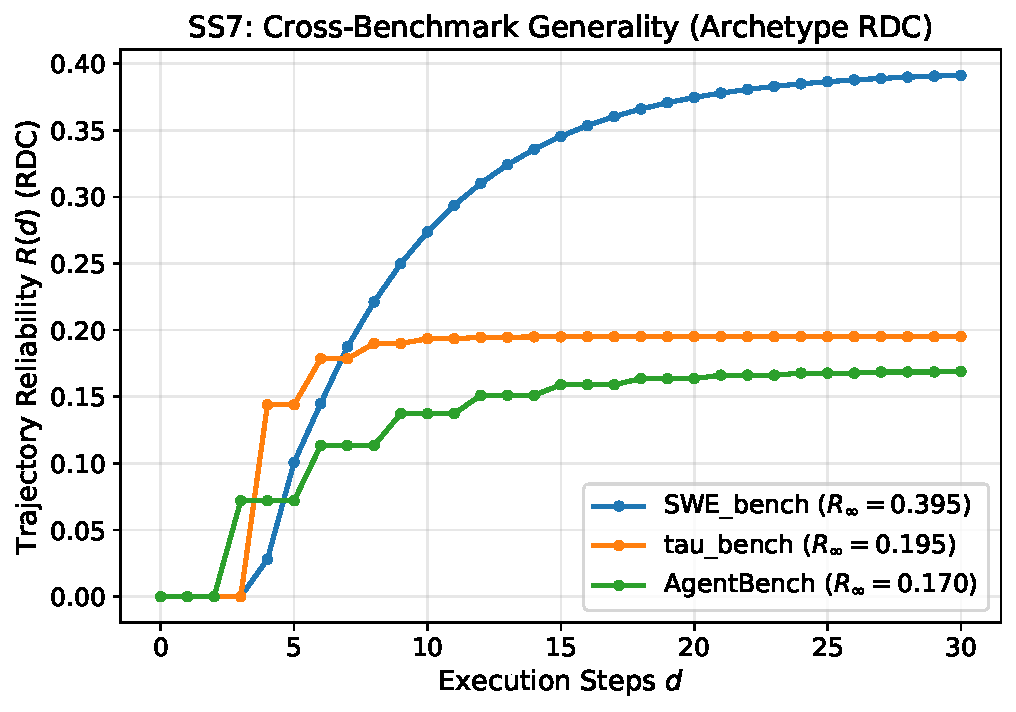
\includegraphics[width=\columnwidth]{../figs/fig_cross_benchmark.pdf}
  \caption{Cross-benchmark archetypes show vocabulary portability:
           RDCs for synthetic state spaces modeling SWE-bench,
           $\tau$-bench, and AgentBench.}
  \label{fig:cross_bench}
\end{figure}

\begin{figure}[!t]
  \centering
  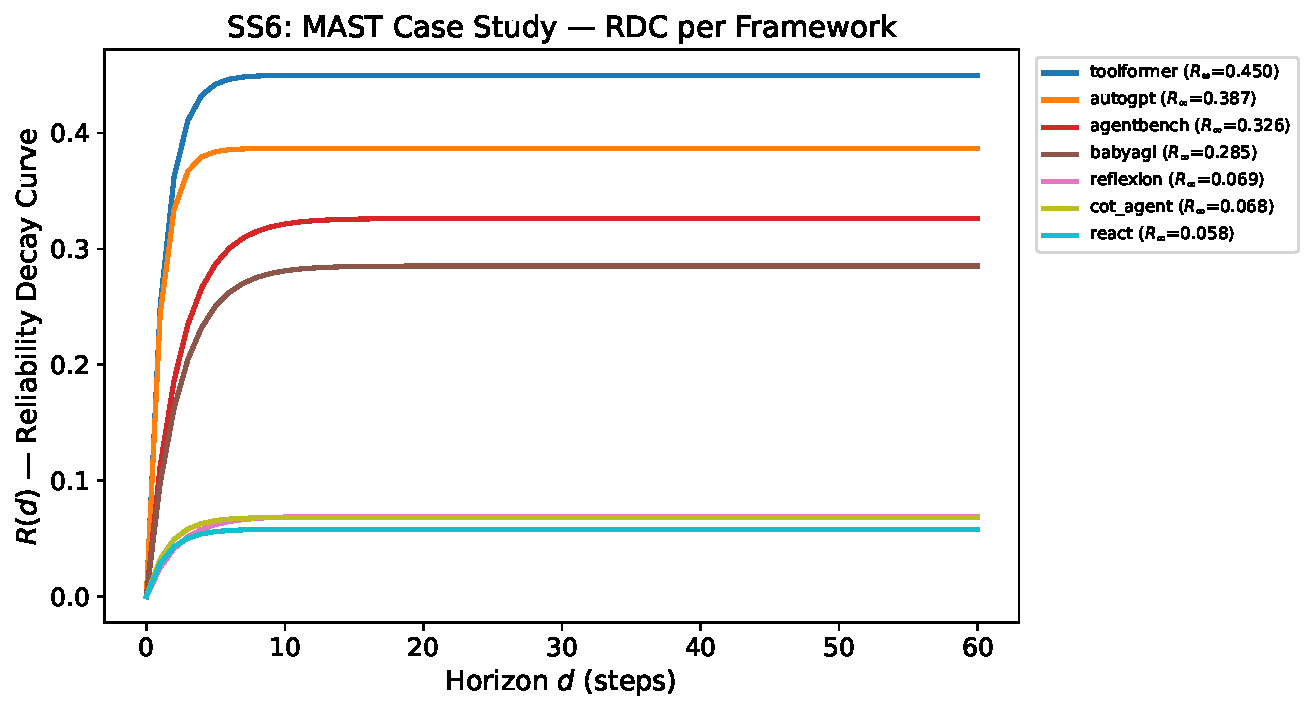
\includegraphics[width=\columnwidth]{../figs/fig_rdc.pdf}
  \caption{SS6 illustrates finite-horizon reliability on MAST-derived
           summaries: reliability decay curves for 7 frameworks ranked
           by $R_\infty$.}
  \label{fig:rdc}
\end{figure}
\fi
%% [END REDUCTION — cross-benchmark archetypes + SS6 RDC figure]

These case studies support a narrow claim: when the diagnostics accept
the trace-to-chain abstraction, the fitted chain provides a coherent
reliability vocabulary for horizons and frameworks, with the limits set
by the available trace representation and the GoF diagnostics.

%% ================================================================

\section{Real Agent-Trace Validation (SS10, SS14)}
\label{sec:ss10}

\subsection{SS10: Does the Certificate Reject?}

The decisive question is whether an \emph{operational} agent trace corpus is
adequately described by a first-order absorbing DTMC and, if not, whether the
composite certificate rejects it. SS10 fits \textsc{TraceToChain} end-to-end
to a real LLM-agent corpus and reports the outcome as-is.

\paragraph{Corpus and provenance.}
We use the publicly released reasoning traces of a SWE-agent submission to the
SWE-bench~Verified leaderboard~\cite{swebench2024} (SWE-agent driving
Claude-4-Sonnet), which archives one \texttt{.traj} file per instance recording
the per-step \texttt{action}, \texttt{observation}, and \texttt{state}; the
SWE-bench \texttt{resolved} verdict gives the ground-truth label. We harvested
$479$ instances ($324$ resolved, $155$ unresolved; $29{,}504$ steps). A
rule-based featurizer---as in SS7---maps each step to a semantic action
category by parsing the issued command (stripping \texttt{cd~\ldots~\&\&}
wrappers and recording the file-editor sub-command), giving the alphabet
\{\textsc{view}, \textsc{edit}, \textsc{execute}, \textsc{search},
\textsc{inspect}, \textsc{vcs}, \textsc{submit}, \textsc{fileop},
\textsc{none}, \textsc{other}\}. No trajectory text beyond these features is
used; corpus and harvester are in the artifact.

\paragraph{Protocol.}
We follow the SS9 protocol: the corpus is split $50/50$ \emph{before}
featurization and clustering, \textsc{TraceToChain} is fitted on the fit half
only, and the held-out half drives the Kolmogorov--Smirnov (KS) first-passage
test and the empirical RDC. To keep Ward clustering tractable on a single
machine we first draw a deterministic sub-sample of the corpus (uniform
without replacement under a fixed seed) and split \emph{that}; the reported
run uses $160$ traces in total, i.e.\ $80$ fit and $80$ test.

\paragraph{Result: the certificate rejects.}
Table~\ref{tab:ss10} summarizes the fit. The clustering itself is clean,
recovering $m{=}7$ well-separated states (silhouette $0.80$): six are pure
single-category states (\textsc{execute}, \textsc{view}, \textsc{edit},
\textsc{search}, \textsc{vcs}, \textsc{submit}) and the seventh pools the
low-frequency \textsc{fileop}, \textsc{none}, and \textsc{other} steps. Despite this, the \emph{composite
certificate rejects the first-order absorbing DTMC}: the AIC layer strongly
prefers a second-order chain ($\Delta_{\mathrm{AIC}} = +817$, so the
first-order model is \emph{not} selected), the held-out first-passage KS test
rejects with $D_{\mathrm{KS}} = 0.39$, $p < 10^{-4}$, and the analytic RDC
departs from the held-out empirical RDC by $L_\infty^{\mathrm{RDC}} = 0.26$.
The rejection is stable at total sub-sample sizes of $120$ and $160$ traces
and under both featurizations (KS $p < 10^{-4}$ throughout);
\S\ref{sec:robustness} reports the full $\Delta_{\mathrm{AIC}}$ spread across
the configuration grid.

% Auto-generated by SS10_swebench_real.py -- do not edit by hand.
\begin{table}[!t]
\centering
\caption{SS10: \textsc{TraceToChain} on $479$ real SWE-agent trajectories.}
\label{tab:ss10}
\begin{tabular}{lr}
\toprule
\textbf{Quantity} & \textbf{Value} \\
\midrule
Instances used (succ/fail) & 479 (324/155) \\
Agent steps & 29504 \\
Fit / test traces & 80 / 80 \\
Recovered states $m$ & 7 \\
Silhouette & 0.801 \\
$\Delta_{\mathrm{AIC}}$ (1st$-$2nd) & +817.2 \\
First-order preferred (AIC) & no \\
Held-out KS $D$ & 0.393 \\
Held-out KS $p$ & 0.0000 \\
$L_\infty^{\mathrm{RDC}}$ (held-out) & 0.260 \\
\midrule
\textbf{Composite verdict} & \textbf{REJECT} \\
\bottomrule
\end{tabular}
\end{table}


%% [REDUCTION] fig:ss10 (RDC mismatch) is suppressed for the 12-page body: Table~\ref{tab:ss10}
%% gives $L_\infty^{\mathrm{RDC}}$ and Fig.~\ref{fig:ss14} (left) shows the same
%% first-passage mismatch. Figure retained in the artifact.
\iffalse
\begin{figure}[!t]
  \centering
  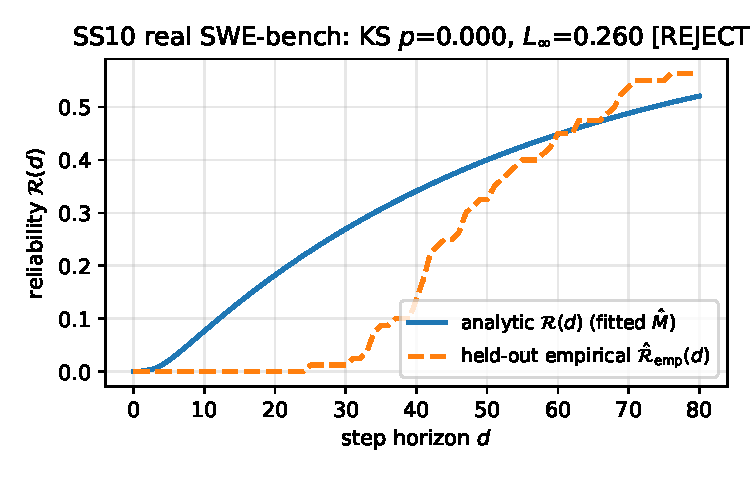
\includegraphics[width=\columnwidth]{../figs/fig_ss10_swebench.pdf}
  \caption{SS10 (real SWE-agent traces): the analytic RDC from the fitted
           first-order chain $\mathcal R(d)$ does \emph{not} track the held-out
           empirical RDC $\hat{\mathcal R}_{\mathrm{emp}}(d)$
           ($L_\infty^{\mathrm{RDC}}=0.26$, KS $p<10^{-4}$). The composite
           certificate rejects the first-order absorbing-DTMC abstraction for
           this corpus.}
  \label{fig:ss10}
\end{figure}
\fi


\paragraph{Interpretation.}
Real SWE-agent trajectories carry history dependence (retries, tool state,
accumulated context) that a first-order chain over action categories does not
capture; the AIC$\,\wedge\,$KS certificate detects exactly this and
\emph{withholds} the first-passage interpretation, in line with the ``reject
if GoF fails'' discipline of \S\ref{sec:threats}. SS10 therefore validates the
safeguard on operational data: on this corpus one should not report
$\mathcal R(d)$ from a first-order DTMC, while the estimator-level recovery
guarantees of SS9 and the diagnostic behavior of SS7 remain intact. \S\ref{sec:ss14} then takes the
constructive next step: it localizes the misfit to the success-time
distribution, shows that $R_\infty$ is nonetheless recovered accurately, and
identifies the duration-aware model needed for horizon queries.

\subsection{SS14: What the Audit Accepts}
\label{sec:ss14}

The natural follow-up is to ask which model the data \emph{does} support and
which reliability outputs are trustworthy. SS14 answers both; because the base
states are the action categories themselves, no clustering is needed and we use
the full $479$-trace corpus ($50/50$ fit/test).

\paragraph{The misfit is in duration, not order.}
An order-$k$ Markov chain is a first-order absorbing chain on category
$k$-tuples, so we can lift the corpus to $k\in\{1,2,3\}$ and to a duration-aware
phase-type variant (state $=$ (category, coarse progress stage)) and re-run the
held-out success first-passage KS test. Table~\ref{tab:ss14} reports the order
lifts: the timing is rejected at \emph{every} order ($p<10^{-3}$), and a
higher order does not help (it worsens with data sparsity). The reason is
visible in Figure~\ref{fig:ss14} (left): real successful runs are
\emph{concentrated} (held-out $10$--$90$th percentile $34$--$86$ steps, median
$54$, with a floor near $30$), whereas a category-Markov chain produces a
geometric-shaped first-passage time with mass near zero and a long tail. The
phase-type lift narrows the gap substantially (KS $D$ from $0.34$ to $0.29$)
by letting the per-step hazard depend on progress, but does not fully close it.
The non-Markovian structure of real agent traces is therefore primarily in the
\emph{success-time distribution}, and a genuinely duration-aware model
(semi-Markov / phase-type with a learned holding-time law) is the indicated
remedy---a sharper diagnosis than ``the chain does not fit.''

% Auto-generated by SS14_higher_order.py
\begin{table}[!t]\centering
\caption{SS14: order-$k$ lifts of the real SWE-bench corpus.}
\label{tab:ss14}
\begin{tabular}{rrrrrl}
\toprule
order $k$ & states & $R_\infty$ & KS $D$ & KS $p$ & verdict \\
\midrule
1 & 10 & 0.656 & 0.341 & 0.000 & REJECT \\
2 & 82 & 0.600 & 0.364 & 0.000 & REJECT \\
3 & 318 & 0.546 & 0.425 & 0.000 & REJECT \\
\bottomrule
\end{tabular}
\end{table}


\paragraph{The asymptotic reliability is accepted, and the metric/perturbation
use cases work on real data.}
Crucially, the audit does not reject everything: it separates the
trustworthy outputs from the untrustworthy ones. The fitted chain's asymptotic
reliability $R_\infty$ (eventual success probability) \emph{matches the
held-out empirical pass rate} on the full $479$-trace corpus: at first order
$R_\infty = 0.656$ versus an observed pass rate of $0.683$, i.e.\ within
$0.027$
(Figure~\ref{fig:ss14}, right; the parsimonious first-order chain is best, as
higher orders overfit $R_\infty$). Two of the three motivating use cases
therefore pay off directly on real traces, because they depend on $R_\infty$
rather than on the rejected timing:
\emph{metric reconciliation}---from the single fitted $R_\infty$ we read
$\mathrm{pass}@1 = 0.66$, $\mathrm{pass}@5 = 0.995$, $\mathrm{pass}^5 = 0.12$,
reconciling the three conventions without a third denominator; and
\emph{fallback-tool perturbation}---rerouting $10\%$ of each state's failure
mass to success yields $\Delta R_\infty = +0.034$. Because this moves mass
into $R_\oplus$ rather than within $Q$, it falls outside the scope of
Proposition~\ref{thm:perturb} and is computed as an \emph{exact}
re-evaluation of Proposition~\ref{thm:closed} on the modified chain; either
way it needs no benchmark rerun. The third use case, horizon extrapolation $\mathcal R(d)$, is
exactly the quantity the KS test rejects, so the audit \emph{withholds} it and
flags that a duration-aware model is required before reporting it.

\begin{figure}[!t]
  \centering
  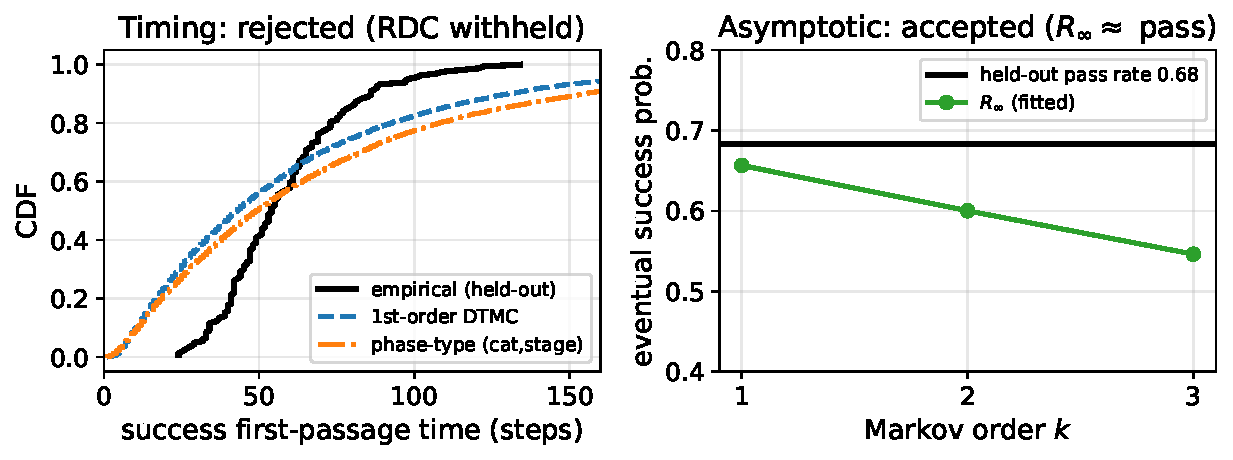
\includegraphics[width=\columnwidth]{../figs/fig_ss14_realfit.pdf}
  \caption{SS14: success first-passage CDF (left) and $R_\infty$ by
           Markov order (right) on real SWE-agent traces.}
  \label{fig:ss14}
\end{figure}

On real agent traces the framework is therefore neither uniformly valid nor
uniformly useless---the intended behavior of an estimation-and-audit pipeline.

\section{Cross-Benchmark Real-Data Validation (SS15)}
\label{sec:ss15}

A single corpus is one verdict. SS15 tests whether the SS10/SS14 pattern
\emph{generalizes} to a second, very different real benchmark---the
conversational tool-use benchmark $\tau$-bench---across two models and two
task domains.

\paragraph{Corpus and provenance.}
We use the publicly released $\tau$-bench trajectory
archive~\cite{taub2024}: Claude-3.5-Sonnet and GPT-4o on the retail and
airline domains, $1{,}980$ episodes in total, each carrying the task reward as
a ground-truth success label. The agent's actions are its \emph{assistant
turns}, mapped to five categories---respond, lookup (read-only tool), write
(state-changing tool), handoff, and think---and the episode absorbs by reward.
Since the MLE and the first-passage KS test depend only on transition counts
and the success-length distribution, we retain per-domain sufficient statistics
and ship the extractor in the artifact.

\paragraph{The asymptotic reliability is accepted---on every domain and model.}
For each of the four model$\times$domain runs
($n = 920$, $400$, $460$, and $200$ episodes) and for the pooled corpus, the
fitted first-order $R_\infty$ recovers the held-out empirical pass rate almost
exactly: the mean absolute error across the four runs is $0.0075$, and the
pooled estimate is $0.595$ versus an observed pass rate of $0.597$
($|{\rm err}|=0.002$). Figure~\ref{fig:calibration} places these estimates
alongside the SWE-agent corpus of \S\ref{sec:ss10}. Panel~(a) plots fitted
$R_\infty$ against the held-out pass rate for all five real corpora: every
point lies on the identity line, and the two hardest ($\tau$-bench airline,
$0.42$--$0.46$) sit on it as tightly as the two easiest, so the estimator is
calibrated over the full competence range, not only where agents succeed
often. Panel~(b) shows the residuals: four corpora and the pooled estimate
fall at or below $0.010$, and the largest---SWE-bench at $0.027$---is an order
of magnitude below the $0.27$ spread in pass rates separating the corpora.
They are also one-signed, $R_\infty$ sitting marginally \emph{below} the
observed rate everywhere, consistent with the conservative exit estimates
censoring induces (\S\ref{sec:robustness}). Calibration therefore holds across
a wide difficulty spread and two underlying models---evidence that the
asymptotic output is trustworthy on real agents, not an artifact of one
corpus. Consequently the
metric-reconciliation and perturbation use cases (which depend only on
$R_\infty$) carry over to $\tau$-bench unchanged.

%% [REDUCTION] tab:ss15 is superseded by Fig.~\ref{fig:calibration}, which plots
%% every pass-rate/$R_\infty$ pair and every residual it listed; the remaining
%% columns ($n$, KS $p$) are quoted inline. Table retained in the artifact.
%% % Auto-generated by SS15_taubench.py
\begin{table}[!t]\centering
\caption{SS15: real-data validation on $\tau$-bench ($1{,}980$ episodes).}
\label{tab:ss15}\small
\begin{tabular}{lrrrrr}
\toprule
domain & $n$ & pass & $R_\infty$ & $|{\rm err}|$ & KS $p$ \\
\midrule
sonnet-retail & 920 & 0.69 & 0.69 & 0.01 & 0.000 \\
sonnet-airline & 400 & 0.46 & 0.45 & 0.01 & 0.001 \\
gpt4o-retail & 460 & 0.60 & 0.60 & 0.01 & 0.000 \\
gpt4o-airline & 200 & 0.42 & 0.41 & 0.01 & 0.000 \\
\textbf{POOLED} & \textbf{1980} & \textbf{0.60} & \textbf{0.59} & \textbf{0.00} & \textbf{0.000} \\
\bottomrule
\end{tabular}
\end{table}


\begin{figure}[!t]
\centering
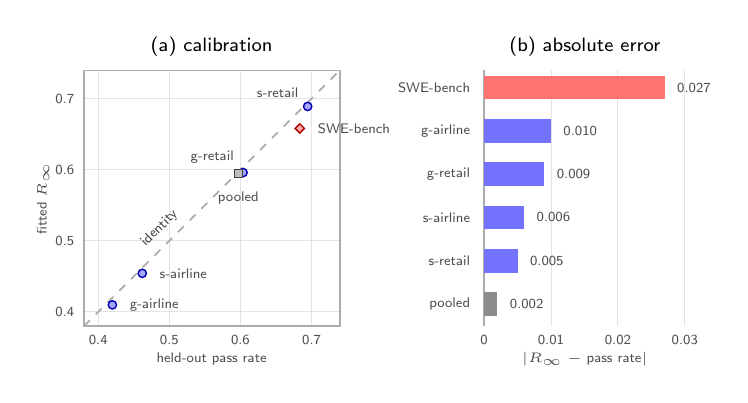
\begin{tikzpicture}[font=\scriptsize\sffamily, >=Stealth,
  ax/.style={draw=gray!65, line width=0.5pt},
  gr/.style={draw=gray!22, line width=0.3pt},
  pt/.style={circle, draw=blue!70!black, fill=blue!35, line width=0.5pt,
             inner sep=0pt, minimum size=3.0pt},
  ptS/.style={diamond, draw=red!65!black, fill=red!35, line width=0.5pt,
              inner sep=0pt, minimum size=3.6pt},
  ptP/.style={rectangle, draw=black!75, fill=black!25, line width=0.5pt,
              inner sep=0pt, minimum size=3.0pt},
  lab/.style={font=\tiny\sffamily, text=black!70}]
\begin{scope}
  \foreach \v in {0.4,0.5,0.6,0.7}{
    \pgfmathsetmacro\c{(\v-0.38)*9.03}
    \draw[gr] (\c,0) -- (\c,3.25);
    \draw[gr] (0,\c) -- (3.25,\c);
    \node[lab, below=0pt] at (\c,0) {\v};
    \node[lab, left=0pt]  at (0,\c) {\v};
  }
  \draw[ax] (0,0) rectangle (3.25,3.25);
  \draw[gray!65, dashed, line width=0.6pt] (0,0) -- (3.25,3.25);
  \node[lab, rotate=45, anchor=south, text=gray!50!black] at (1.10,1.10) {identity};
  \node[pt]  (a) at (2.84,2.79) {};
  \node[pt]  (b) at (0.74,0.67) {};
  \node[pt]  (c) at (2.02,1.95) {};
  \node[pt]  (d) at (0.36,0.27) {};
  \node[ptP] (p) at (1.96,1.94) {};
  \node[ptS] (s) at (2.74,2.51) {};
  \node[lab, above left=-2pt] at (a.north west) {s-retail};
  \node[lab, right=1pt] at (b.east) {s-airline};
  \node[lab, above left=-2pt] at (c.north west) {g-retail};
  \node[lab, right=1pt] at (d.east) {g-airline};
  \node[lab, right=1pt] at (s.east) {SWE-bench};
  \node[lab, below=1.5pt] at (p.south) {pooled};
  \node[lab] at (1.62,-0.42) {held-out pass rate};
  \node[lab, rotate=90] at (-0.52,1.62) {fitted $R_\infty$};
  \node[font=\scriptsize\sffamily] at (1.62,3.55) {(a) calibration};
\end{scope}
\begin{scope}[shift={(5.08,0)}]
  \foreach \v/\c in {0/0, 0.01/0.85, 0.02/1.70, 0.03/2.55}{
    \draw[gr] (\c,0) -- (\c,3.25);
    \node[lab, below=0pt] at (\c,0) {\v};
  }
  \draw[ax] (0,0) -- (0,3.25);
  \foreach \n/\y/\e/\col in {%
      pooled/0.28/0.002/black!45,
      {s-retail}/0.83/0.005/blue!55,
      {s-airline}/1.38/0.006/blue!55,
      {g-retail}/1.93/0.009/blue!55,
      {g-airline}/2.48/0.010/blue!55,
      {SWE-bench}/3.03/0.027/red!55}{
    \pgfmathsetmacro\w{\e*85}
    \fill[\col] (0,\y-0.15) rectangle (\w,\y+0.15);
    \node[lab, right=1pt] at (\w,\y) {\e};
    \node[lab, left=1.5pt] at (0,\y) {\n};
  }
  \node[lab] at (1.28,-0.42) {$|R_\infty-{}$pass rate$|$};
  \node[font=\scriptsize\sffamily] at (1.28,3.55) {(b) absolute error};
\end{scope}
\end{tikzpicture}
\caption{Fitted $R_\infty$ vs.\ held-out pass rate on five real corpora.}
\label{fig:calibration}
\end{figure}


%% [REDUCTION] fig:ss15 (identity-line scatter) is suppressed for the 12-page body:
%% Table~\ref{tab:ss15} lists every point it plots. Retained in the artifact.
\iffalse
\begin{figure}[!t]
  \centering
  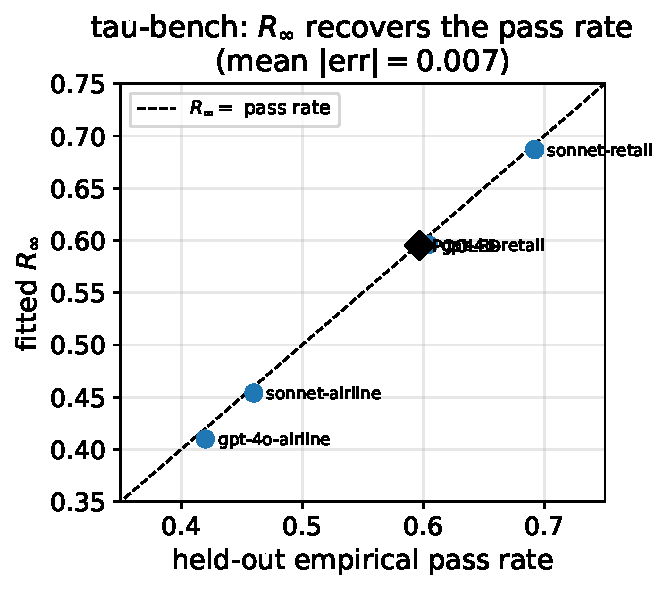
\includegraphics[width=0.62\columnwidth]{../figs/fig_ss15_taubench.pdf}
  \caption{SS15: on real $\tau$-bench traces the fitted $R_\infty$ lies on the
           identity line against the held-out pass rate across both models and
           both domains (mean $|{\rm err}|=0.0075$), replicating the SS14
           SWE-bench finding on a second, conversational benchmark.}
  \label{fig:ss15}
\end{figure}
\fi


\paragraph{The timing behaves exactly as the certificate dictates.}
As on SWE-bench, the success-conditional first-passage KS test rejects the
first-order timing on every domain ($p \le 0.001$ throughout; on sonnet-retail
the empirical median success length is $13$ steps versus a fitted-chain median
of $9$), so the audit
again \emph{withholds} horizon $\mathcal R(d)$ while keeping the accepted
asymptotic and metric outputs. The accept-the-asymptotic /
withhold-the-timing behavior is thus consistent across two independent real
benchmarks, four model$\times$domain corpora, and a wide range of agent
competence.

\section{Robustness and Sensitivity (SS11--SS13)}
\label{sec:robustness}

The diagnostics and estimates depend on three modeling choices---the
clustering that builds the state space, the treatment of censored traces, and
the bootstrap path---and this section reports a controlled sensitivity study
for each.

\paragraph{SS11: clustering and featurization sensitivity.}
Because the certificate is a \emph{joint} test of featurization, clustering,
and the first-order assumption, its verdict could in principle be an artifact
of the clustering. We therefore re-ran the SS10 fit across $18$
configurations: two featurizations (action-category one-hot, with and without
a step-depth feature), three agglomerative linkages (Ward, average, complete),
and three cluster-count caps $k_{\max}\in\{6,8,10\}$. Table~\ref{tab:ss11}
reports the result: the composite verdict is \emph{invariant}, with all $18$
configurations rejecting the first-order absorbing DTMC. The held-out
first-passage KS test rejects ($p<10^{-3}$) in every configuration, including
the three category-only settings at $k_{\max}{=}10$ where the AIC order-test
component alone would accept a first-order chain---so the held-out KS layer is
the binding, clustering-robust component of the certificate, exactly as
intended. The recovered state count $m$ tracks $k_{\max}$ (range $6$--$10$) and
the silhouette varies with featurization, but $\hat R_\infty$ is stable across
all configurations ($0.660$--$0.674$): neither the estimate nor the verdict
moves appreciably with the clustering choice.

\emph{Reconciling the two SWE-bench $R_\infty$ estimates.} The
$\hat R_\infty$ column of Table~\ref{tab:ss11} and the $R_\infty=0.656$ of
SS14 come from different fits of the same benchmark, so each must be read
against its own target: the $160$-trace sub-sample used here has a held-out
pass rate of $0.663$, whereas SS14's full $479$-trace corpus has $0.683$. Read
that way, both are well calibrated---every configuration in the grid lands
within $0.012$ of $0.663$, and SS14 within $0.027$ of $0.683$---so neither
sub-sampling nor the choice of state space distorts the asymptotic estimate.
Because it uses the whole corpus and needs no clustering, the calibration claim
of \S\ref{sec:ss14} and the SWE-bench point of Fig.~\ref{fig:calibration} are
taken from the SS14 fit; $R_\infty$ should in general be reported against the
held-out rate of the split that produced it.

% Auto-generated by SS11_ablation.py
\begin{table}[!t]\centering
\caption{SS11: clustering and featurization ablation ($18$ configurations).}
\label{tab:ss11}\scriptsize
\setlength{\tabcolsep}{3.5pt}
\begin{tabular}{llrrrrrl}
\toprule
feat. & linkage & $k_{\max}$ & $m$ & silh. & $\Delta_{\mathrm{AIC}}$ & KS $p$ & verdict \\
\midrule
cat+depth & ward & 6 & 6 & 0.78 & +872 & 0.000 & REJECT \\
cat+depth & ward & 8 & 7 & 0.80 & +817 & 0.000 & REJECT \\
cat+depth & ward & 10 & 7 & 0.80 & +817 & 0.000 & REJECT \\
cat+depth & average & 6 & 6 & 0.78 & +872 & 0.000 & REJECT \\
cat+depth & average & 8 & 7 & 0.80 & +817 & 0.000 & REJECT \\
cat+depth & average & 10 & 7 & 0.80 & +817 & 0.000 & REJECT \\
cat+depth & complete & 6 & 6 & 0.78 & +872 & 0.000 & REJECT \\
cat+depth & complete & 8 & 7 & 0.80 & +817 & 0.000 & REJECT \\
cat+depth & complete & 10 & 7 & 0.80 & +817 & 0.000 & REJECT \\
cat & ward & 6 & 6 & 0.95 & +872 & 0.000 & REJECT \\
cat & ward & 8 & 8 & 0.99 & +736 & 0.000 & REJECT \\
cat & ward & 10 & 10 & 1.00 & -126 & 0.000 & REJECT \\
cat & average & 6 & 6 & 0.95 & +872 & 0.000 & REJECT \\
cat & average & 8 & 8 & 0.99 & +736 & 0.000 & REJECT \\
cat & average & 10 & 10 & 1.00 & -126 & 0.000 & REJECT \\
cat & complete & 6 & 6 & 0.95 & +872 & 0.000 & REJECT \\
cat & complete & 8 & 8 & 0.99 & +736 & 0.000 & REJECT \\
cat & complete & 10 & 10 & 1.00 & -126 & 0.000 & REJECT \\
\bottomrule
\end{tabular}
\end{table}


\paragraph{SS12: censoring sensitivity.}
The censoring figures reported elsewhere ($\le 10\%$) are mild, and real
deployments may truncate far more aggressively. We took a known ground-truth
absorbing chain ($R_\infty = 0.784$), sampled $600$ trajectories, and refit
\textsc{TraceToChain} after right-censoring a controlled fraction of traces
(truncating at a uniform-random transient step and marking the trace as
censored, neither success nor failure). Under this non-informative censoring the recovered
$\hat R_\infty$ stays within $\approx\!4\%$ of the truth at every level: the
relative bias moves only over $[-4.2\%, -2.6\%]$ across censoring fractions
$0$--$50\%$, against $-3.3\%$ with no censoring at all, so censoring
contributes almost none of the residual. Censored traces still contribute
their observed transient transitions but are correctly excluded from the
absorption counts, so the exit estimates are not materially biased. This
holds for censoring independent of the outcome; \emph{informative} censoring
(e.g.\ a step budget that truncates precisely the long, failure-bound
trajectories) could still bias the estimates, and detecting that regime is
left to future work.

%% [REDUCTION] tab:ss12 is a nearly-flat 7-row column whose every value is
%% quoted inline below; retained in the artifact.
%% % Auto-generated by SS12_censoring.py
\begin{table}[!t]\centering
\caption{SS12: censoring sensitivity on a ground-truth chain ($R_\infty=0.784$).}
\label{tab:ss12}
\begin{tabular}{rrrr}
\toprule
censoring & $\hat m$ & $\hat R_\infty$ & rel.\ bias \\
\midrule
0\% & 5 & 0.758 & -3.3\% \\
5\% & 5 & 0.755 & -3.7\% \\
10\% & 5 & 0.755 & -3.7\% \\
20\% & 5 & 0.764 & -2.6\% \\
30\% & 5 & 0.755 & -3.7\% \\
40\% & 5 & 0.752 & -4.2\% \\
50\% & 5 & 0.756 & -3.6\% \\
\bottomrule
\end{tabular}
\end{table}


\paragraph{SS13: bootstrap path and uncertainty understatement.}
The intervals of \S\ref{sec:uq} are reported via the fast bootstrap path, which
holds the target clustering fixed (nearest-centroid reassignment of resampled
steps). The module also implements a full re-cluster bootstrap
(\texttt{fast=False}) that re-runs Ward clustering on every resample and so
additionally captures clustering instability. On a controlled $250$-trace
corpus the full re-cluster path gives transition intervals whose median
half-width is $\approx\!4.7\times$ that of the fixed-clustering path ($0.158$
vs.\ $0.034$). The fixed-clustering intervals therefore understate total
uncertainty and should be read as a lower bound conditioned on the chosen
clustering; we recommend reporting the full re-cluster path (or both) when
clustering stability is in question.

\section{Threats to Validity}
\label{sec:threats}

The main threat is overinterpreting the fitted abstraction. The chain
remains a reliability model for specified trace features under
specified diagnostics, not a universal model of agent behavior, so the
estimates should be read conditionally.

\paragraph{Construct validity (state construction).}
Mapping trajectories to a DTMC aggregates over memory, tool state, and
context, and no single mapping is canonical.
\S\ref{sec:state_construction} gives a reproducible construction whose
output is \emph{tested} by Algorithm~\ref{alg:gof}: SS7 checks the
protocol on known synthetic chains and SS9 checks controlled fit/test
recovery. These establish statistical adequacy for the chosen features,
not uniqueness of $\phi$. If GoF rejects, first-passage interpretation
should stop until traces are segmented, re-featurized, or modeled with
a richer process; semi-Markov or hidden Markov models (HMMs) are the
natural next steps. We therefore recommend reporting
$(\phi, m, p_{\mathrm{KS}}, \Delta_{\rm AIC})$ with each estimate.

\paragraph{Estimator sensitivity.}
The composite verdict is invariant across the $18$ configurations of
SS11, and $\hat R_\infty$ varies only over $[0.660,0.674]$ there. Even
so, $R_\infty$ is a property of the split that produced it---sub-sampling
moves the held-out target as well as the estimate---so it must always be
reported against the held-out rate of its own split.

\paragraph{Empirical scope of SS9.}
SS9 uses synthetic traces from a true absorbing chain with noisy
one-hot emissions, so its held-out KS test evaluates controlled
recovery by the trace-to-chain pipeline (featurizer + clustering + MLE)
rather than the full modeling class on unprocessed benchmark data;
\S\ref{sec:ss10}--\ref{sec:ss15} supply the real-trace counterpart.

\paragraph{Independence assumption.}
The pass$^k$ and pass$@k$ identities require i.i.d.\ trials
(A\ref{A:iid}), which can fail under temperature-0 sampling or shared
prefixes. Theorem~\ref{thm:corr} and Corollary~\ref{cor:diag} quantify
the resulting bias and provide a diagnostic.

\paragraph{External validity.}
The MAST case study covers 7 frameworks, so its conclusions may not
generalize to other agents, tasks, or trace distributions; SS6 is
therefore framed as illustrative rather than confirmatory.

\paragraph{NHPP-limit scope.}
The NHPP limit applies under rare-failure scaling
($\varepsilon\to 0$, $d\to\infty$); in high-failure regimes
($\varepsilon > 0.1$) the exact closed form of
Proposition~\ref{thm:closed} should be used instead. That is the common
case for deployed agents---the SWE-agent corpus of \S\ref{sec:ss10}
fails on roughly $32\%$ of tasks ($155/479$)---so the
Goel--Okumoto/NHPP limit is best treated as a conceptual bridge to
reliability-growth theory rather than an estimator at these rates.

%% ================================================================

\section{Discussion}
\label{sec:disc}

For benchmark authors, SRE teams, and method developers, the fitted
chain provides a shared reliability object at the trace level: it
supports first-passage metrics with uncertainty, horizon and
perturbation queries, and diagnostics that can reject an inadequate
abstraction. SS9 (Table~\ref{tab:heldout-ss9}) shows that, once the
trace-to-chain step is specified and checked, $\hat M$ tracks held-out
first-passage behavior to within $L_\infty^{\mathrm{RDC}}\le 0.053$
across seven frameworks. This does not replace benchmarks or incident
analysis; it shows how benchmark-style trace corpora can support
auditable reliability answers while also flagging when the abstraction
is too weak for them. The practical requirement is to fit the chain,
report uncertainty, run GoF, and withhold first-passage conclusions
when the checks fail.

The real-data studies make this concrete and show the audit is
\emph{selective} rather than all-or-nothing: across SWE-bench (SS10,
SS14) and $\tau$-bench (SS15) it accepts the asymptotic reliability but
rejects the first-order RDC timing, while SS11--SS13
(\S\ref{sec:robustness}) show the verdict survives the clustering
choice even where the point estimate does not. The value of the fitted
chain on real traces is thus real but \emph{partial}, and the audit is
what makes it safe by saying which part to trust.

The clearest next step, identified by the data rather than assumed, is a
duration-aware model: SS14 localizes the misfit to the success-time
distribution, so semi-Markov holding times (or a learned phase-type
duration law) are the indicated route to restoring horizon queries.
Further directions include HMM reliability under partial observability,
online estimation of $Q$, integration with PRISM and Storm, and
mixture-chain models for cross-trial correlation~\cite{spaeh2024}.

%% ================================================================

\section{Conclusion}
\label{sec:conc}

LLM-agent teams already collect execution traces, but scalar metrics
alone do not answer deployment reliability questions.
\textsc{TraceToChain} turns those traces into an audited absorbing-chain
model, combining a composite AIC$\,\wedge\,$KS certificate,
Dirichlet-posterior and bootstrap intervals, and a strict held-out
protocol, and it recasts pass$@k$, pass$^k$, and the RDC as projections
of a single success-time distribution. On seven controlled MAST-style
frameworks the analytic and held-out empirical RDCs agree to
$\max L_\infty^{\mathrm{RDC}}=0.053$ with KS acceptance on $7/7$
corpora. On $2{,}459$ real episodes from two independent benchmarks the
certified asymptotic reliability recovers the held-out pass rate to
within $0.03$ on SWE-bench and to a mean of $0.0075$ across four
$\tau$-bench corpora, delivering metric reconciliation and closed-form
perturbation answers on real agents with no benchmark rerun, and the
certificate marks precisely which further outputs its evidence
supports. The verdict is invariant across $18$ clustering configurations, and
$\hat R_\infty$ stays within $4\%$ of a synthetic ground truth up to
$50\%$ censoring. The result is a reliability model that reports not
only a number but the evidence that licenses it.

%% ================================================================


\balance
\bibliographystyle{IEEEtran}
\bibliography{refs}

%% ----------------------------------------------------------------
%% [REDUCTION 2026-04-24] The Extended Proofs appendix is suppressed
%% from the 12-page body. All T1--T6 proofs and extended remarks are
%% retained in the reproducibility artifact under
%% \texttt{proofs/T1.tex}--\texttt{proofs/T6.tex}.
%% ----------------------------------------------------------------
\iffalse
\appendix
\section{Extended Proofs}
\label{app:proofs}

Full proofs of Propositions~\ref{thm:shape}--\ref{thm:mixing} are
provided in the companion artifact at
\texttt{proofs/T4.tex}--\texttt{proofs/T6.tex}. The main text
includes proof sketches only due to the 12-page limit.
\fi

\end{document}
